\documentclass[pdftex,a4paper,12pt,DIV12,oneside,bibtotocnumbered,idxtotoc,halfparskip,chapterprefix]{scrbook}

\usepackage{amssymb}
\usepackage{fancyhdr}
\usepackage{flafter}
\usepackage{float}
\usepackage[T1]{fontenc}
\usepackage[scaled=.90]{helvet}
\usepackage[pdftex]{hyperref}
\usepackage[latin1]{inputenc}
\usepackage{mathptmx}
\usepackage{rotating}
\usepackage{setspace}
\usepackage{url}
\usepackage{xcolor}

% Page Layout
\headheight = 0.05\textheight
\pagestyle{fancy}
\fancyhead{}
\fancyfoot{}
\renewcommand{\headrulewidth}{0.4 pt}
\renewcommand{\footrulewidth}{0.4 pt}
\fancyhead[L]{\small Sebastian Bergmann}
\fancyhead[R]{\small Design and Implementation of a Workflow Engine}
\fancyfoot[L]{\small \nouppercase{\footnotesize{\leftmark}}}
\fancyfoot[R]{\small \thepage}
\parindent0em

% Font
\setkomafont{sectioning}{\normalfont\bfseries}
\setkomafont{captionlabel}{\normalfont\bfseries}
\setkomafont{pagehead}{\normalfont\itshape}
\setkomafont{descriptionlabel}{\normalfont\bfseries}

% Listings
\usepackage[savemem]{listings}
\definecolor{lbcolor}{rgb}{0.85,0.85,0.85}
\lstset{numbers=left,
        stepnumber=1,
        numbersep=5pt,
        numberstyle=\tiny,
        breaklines=true,
        breakautoindent=true,
        postbreak=\space,
        tabsize=2,
        basicstyle=\ttfamily\footnotesize,
        showspaces=false,
        showstringspaces=false,
        extendedchars=true,
        backgroundcolor=\color{lbcolor}}

% PGF / TikZ
\usepackage{tikz}
\usetikzlibrary{arrows,automata,backgrounds,petri,shapes}
\tikzstyle{node}=[circle,draw=gray!50,fill=gray!20,thick]
\tikzstyle{activity}=[rectangle,draw=gray!50,fill=gray!20,thick]
\tikzstyle{who}=[rectangle,draw=blue!50,fill=blue!20,thick]
\tikzstyle{what}=[circle,draw=green!50,fill=green!20,thick]
\tikzstyle{how}=[rectangle,draw=yellow!50,fill=yellow!20,thick]
\tikzstyle{place}=[circle,thick,draw=gray!75,fill=gray!20,minimum size=6mm]
\tikzstyle{transition}=[rectangle,thick,draw=black!75,fill=black!20,minimum size=4mm]

% Metadata
\author{Sebastian Bergmann}
\title{Design and Implementation of a Workflow Engine}
\hypersetup{pdfauthor={Sebastian Bergmann},
            pdftitle={Design and Implementation of a Workflow Engine},
            pdfkeywords={PHP, Graph-Oriented Programming, Workflow Management},
            pdfsubject={PHP, Graph-Oriented Programming, Workflow Management},
            pdfcreator={LaTeX, Doxygen, KOMA-Script, PGF, TikZ},
            pdfproducer={LaTeX, Doxygen, KOMA-Script, PGF, TikZ},
            bookmarks,
            pdfstartview=FitH,
            pdfpagelayout=OneColumn}

\begin{document}

\frontmatter
\begin{titlepage}
\begin{center}


\includegraphics[width=6cm]{figures/unibonn-logo}\\[5mm]

{\bf Rheinische Friedrich-Wilhelms-Universit�t}\\[5mm]
{Institut f�r Informatik III \\ Prof.~Dr.~Armin~B.~Cremers}\\[3cm]

{\LARGE\bf Design and Implementation of a Workflow Engine}\\[3cm]

{\bf Diplomarbeit von}\\[5mm]
{Sebastian Bergmann \\
Aulgasse 14 \\
53721 Siegburg \\[5mm]
E-Mail: sb@sebastian-bergmann.de\\[5mm]
Matrikelnummer: 1247261}\\[2cm]

\begin{tabular}[h]{rl}
1. Gutachter: & Prof.~Dr.~Armin~B.~Cremers\\
2. Gutachter: & Prof.~Dr.~Rainer~Manthey\\
\end{tabular}\\[2cm]

\begin{tabular}[h]{rl}
Tag der Abgabe:        & 13. Februar 2007\\
Letzte Aktualisierung: & 23. Januar 2008\\
\end{tabular}
\end{center}

\end{titlepage}

\pagenumbering{roman}
\thispagestyle{empty}

\addcontentsline{toc}{section}{Manifesto}
\addcontentsline{toc}{section}{License}
\noindent
Manifesto\\
\\
Except where indicated otherwise, this thesis is my own original work.\\
\\[1cm]
Sebastian Bergmann\\
\\[9cm]
This thesis is published under the Creative Commons Attribution 2.0 Germany license.\\
\\
You are free:

\begin{itemize}
\item to copy, distribute, display, and perform the work
\item to make derivative works
\item to make commercial use of the work
\end{itemize}

Under the following conditions:

\begin{itemize}
\item {\bf Attribution}. You must attribute the work in the manner specified by the author or licensor.
\item For any reuse or distribution, you must make clear to others the license terms of this work.
\item Any of these conditions can be waived if you get permission from the copyright holder.
\end{itemize}

Your fair use and other rights are in no way affected by the above.

\cleardoublepage
\thispagestyle{empty}
\onehalfspacing
\addcontentsline{toc}{section}{Abstract}
\noindent
{{\LARGE\bf Abstract}\\
\\
\\
This thesis discusses the design and implementation of a software component
that faciliates the specification, management, and execution of so-called
workflows.\\
The discussion of this component's design includes the semantics and syntax of
the underlying workflow model as well as the actual software design. The
former builds upon the \emph{Workflow Patterns} \cite{BK03} terminology, the
latter on the concepts of a \emph{Workflow Virtual Machine} \cite{SF04} and
the idea that a workflow system should be comprised of loosely coupled
components \cite{DAM01,DG95,PM99}.\\
\\
\\
Diese Diplomarbeit behandelt den Entwurf und die Implementierung einer
Softwarekomponente f�r die Definition, Verwaltung und Ausf�hrung von 
Spezifikationen so genannter Workflows.\\
Die Diskussion des Entwurfs dieser Komponente behandelt Semantik und Syntax
des zugrunde liegenden Workflow-Modells ebenso wie das eigentliche
Software-Design. Ersteres baut auf der Terminologie der \emph{Workflow Patterns}
\cite{BK03} auf, letzteres auf dem Konzept einer \emph{Workflow Virtual Machine}
\cite{SF04} und der Idee, dass ein Workflow-System aus lose gekoppelten
Komponenten aufgebaut sein sollte \cite{DAM01,DG95,PM99}.\\
\\
Diese Diplomarbeit wurde in englischer Sprache verfasst.

\cleardoublepage
\tableofcontents
\addcontentsline{toc}{section}{List of Figures}
\listoffigures
\cleardoublepage
\pagestyle{fancy}
\pagenumbering{arabic}
\mainmatter

\addcontentsline{toc}{chapter}{Introduction}
\chapter*{Introduction}

\section*{Problem Statement and Goal}

This thesis has the design and implementation of a workflow engine as its goal.
This goal has motivations from both academia and industry that were represented
by the two supervising institutions, the Institute of Computer Science of the
University of Bonn, Germany and eZ~Systems~AS, respectively.

The topic of this diploma thesis was set up by eZ~Systems~AS in Skien,
Norway. The company is the creator of eZ~Publish, an Open Source Enterprise
Content Management System, and eZ~Components, a components library for PHP~5.
As we will see in Chapter~\ref{chapter-Requirements}, eZ~Systems~AS is in need
of a flexible and reusable workflow engine component, written in the PHP
programming language, that can be used in the development of the next version
of their eZ~Publish~ECMS. Of academic interest is how research such as
\cite{BK03,DAM01,PM99,SF04} can be put to use for the design and
implementation of such a software component.

The goal of this thesis is therefore to \emph{review the relevant literature},
to \emph{find a suitable workflow model} as the foundation for the
\emph{design and implementation of a workflow engine}, and to \emph{evaluate
the resulting software component} with regard to the industry requirements
set up by eZ~Systems~AS.

\section*{Structure}

Chapter~\ref{chapter-ProblemDomain} gives an introduction to the problem domain
of Enterprise Content Management and Workflow Management.
Chapter~\ref{chapter-WorkflowSemantics} presents Petri nets as a formal way and
workflow patterns as a more pragmatic way to define the semantics of a workflow
model.

Chapter~\ref{chapter-Technology} gives an introduction to the technology stack
(PHP, eZ~Publish, eZ~Components) that is relevant to and used by the software
that has been implemented as part of this thesis.
Chapter~\ref{chapter-Requirements} discusses the requirements that lead to the
development of this software.

Chapter~\ref{chapter-WorkflowModel} presents the semantics and syntax of the
workflow model that is the foundation for the software.
Chapter~\ref{chapter-DesignAndImplementation} discusses the design and
implementation of the software.

This paper concludes with an evaluation of the software
(Chapter~\ref{chapter-Evaluation}), a comparison to related work, and an
outlook on future work (Chapter~\ref{chapter-Conclusion}).

\section*{Acknowledgements}
\thispagestyle{empty}

I would like to thank Prof. Dr. Armin B. Cremers for making it possible that
I could do my thesis in cooperation with eZ~Systems~AS and Dr. Stefan
L�ttringhaus-Kappel for being my thesis advisor. I would like to thank
everyone at eZ~Systems~AS for the great time I had in Norway.

Finally, I would like to express my appreciation for the people involved in
the development of the free software that is discussed in this paper (PHP,
eZ~Publish, eZ~Components) and was used to typeset (\LaTeX, Dia, Doxygen,
GraphViz, KOMA-Script, PGF, Ti\emph{k}Z) this paper.

\chapter{Problem Domain}
\label{chapter-ProblemDomain}

This chapter gives an introduction to the problem domain of Enterprise Content
Management and Workflow Management.

\section{Enterprise Content Management}

The meaning of the term ''Enterprise Content Management'' can be approached
gradually by looking at the three words that make it up:

\begin{itemize}
\item \textbf{Enterprise} refers to the employees of an enterprise with access
      and editing rights.
\item \textbf{Content} refers to arbitrary content stored in the electronic
      systems of an enterprise.
\item \textbf{Management} refers to a software system for the administration,
      control, and processing of content in an enterprise, both internally
      (in an intranet, for example) and externally (on the internet, for
      example).
\end{itemize}

The Association for Information and Image Management (AIIM) defines
Enterprise Content Management (ECM) as

\begin{quote}
\emph{the technologies used to capture, manage, store, preserve, and deliver
content and documents related to organizational processes. ECM tools and
strategies allow the management of an organization's unstructured information,
wherever that information exists} \cite{AIIM}.
\end{quote}

The usage scenarios of eZ~Publish (see Section~\ref{section-eZPublish}), for
example, range from blogs and personal websites to community portals, company
websites, webshops, business process management, enterprise resource planning,
and document management in both governmental institutions and corporate
environments.

\section{Workflow Management}

The Workflow Management Coalition (WfMC) describes workflow management as

\begin{quote}
\emph{the automation of a business process, in whole or parts, where
documents, information or tasks are passed from one participant to another to
be processed, according to a set of procedural rules} \cite{RA01}.
\end{quote}

Georgakopoulos et. al. define workflow management as a

\begin{quote}
\emph{technology supporting the reengineering of business and information
processes. It involves: (1) defining \emph{workflows}, i.e., describing
those aspects of a process that are relevant to controlling and
coordinating the execution of its tasks [...], and (2) providing for fast
(re)design and (re)implementation of the processes as business needs and
information systems change} \cite{DG95}.
\end{quote}

Workflow management systems are software systems that enable workflow
management.

There are two kinds of workflow management systems: those that are
\emph{activity-based} and those that are \emph{entity-based}. The former have
their focus on the activities that are to be completed throughout the workflow,
the latter focus on entities, such as documents, that are processed by a
workflow \cite{FG02}.

The documentation of the OpenFlow workflow management system \cite{OPENFLOW}
summarizes the purpose of an activity-based workflow management system as
\emph{answering the question ''who must do what, when and how''}:

\begin{itemize}
\item The workflow definition (or \emph{workflow schema}) defines the sequence
      of activities that are to be carried out. It specifies \emph{what}
      should be done and \emph{when} by the definition of activities
      (represented by the \emph{nodes} of a directed graph) and transitions
      (represented by the \emph{edges} of a directed graph).

\item An activity (the \emph{what} part of the issue) represents
      something to be done: reviewing a document, publishing a document,
      placing an order, sending an e-mail, and so on.

\item Transitions define the appropriate sequence of activities for a
      process (the \emph{when} part of the issue).

\item Each activity will have an associated application designed to
      carry out the job: the \emph{how} part.

\item The \emph{who} part is generally the user or system assigned to carry
      out the activity, through its application.
\end{itemize}

Figure~\ref{figure-SampleWorkflow} shows a sample workflow that illustrates
this: The green nodes represent the activities that are to be completed
throughout the workflow. The red edges between the nodes represent the control
flow. Depending on the input that is provided by a user with the appropriate
access rights (blue), the \emph{branch} nodes chooses one of two possible
actions that are encapsulated by so-called \emph{service objects} (yellow).
After one of those two possible actions has been performed, the \emph{merge}
nodes merges the control flow again.

The interaction with the user (to receive input, for instance) is performed
through a so-called \emph{worklist} interface. The software system into
which the workflow management system is integrated queries the workflow
system whether a workflow instance is waiting for input that can be
provided by the current user. The user can then provide the input through
the worklist interface.

\begin{figure}[hbtp]
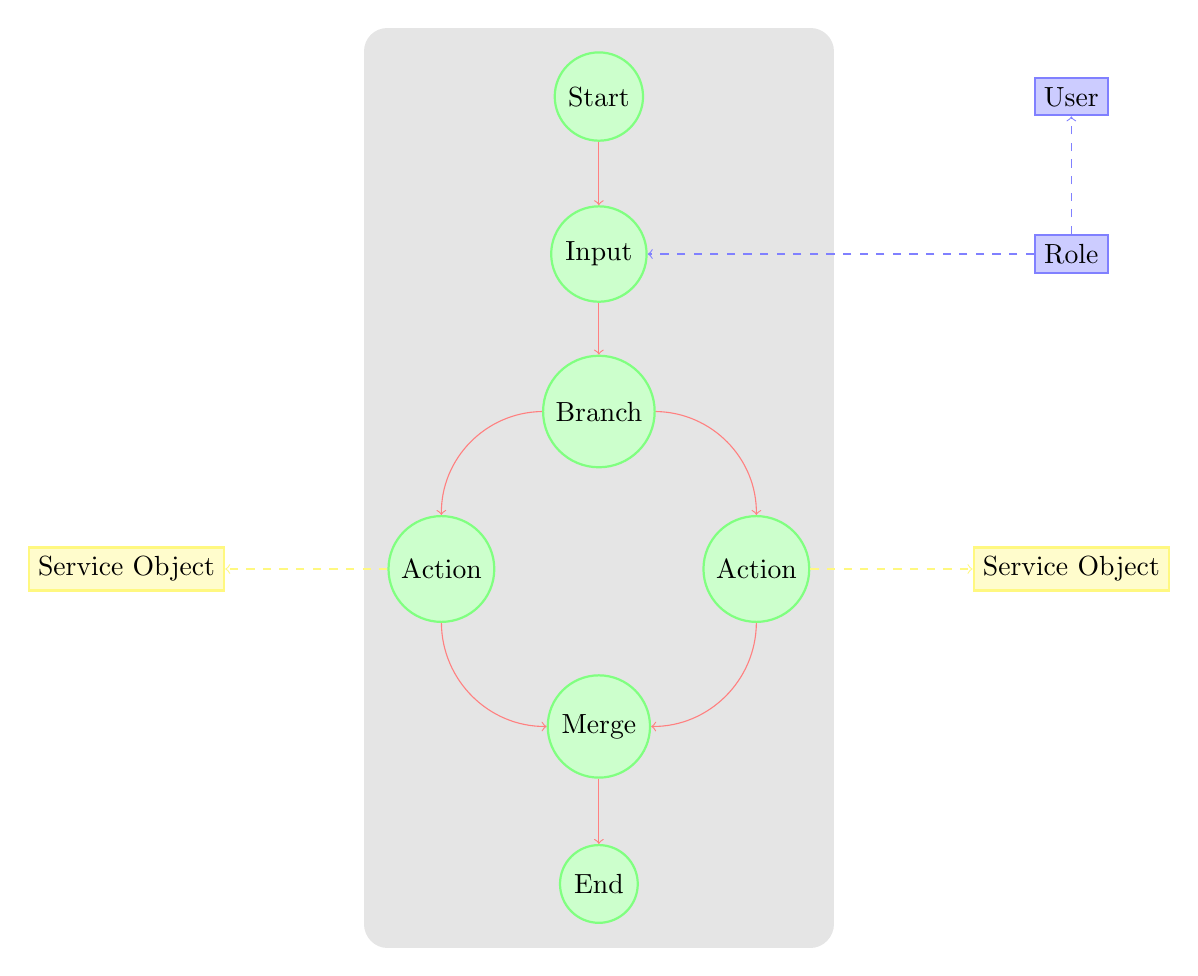
\begin{tikzpicture}
  \node at ( 0, 6) [what] (Start) {Start};
  \node at ( 0, 4) [what] (Input) {Input};
  \node at ( 0, 2) [what] (Branch) {Branch};
  \node at (-2, 0) [what] (ActionA) {Action};
  \node at ( 2, 0) [what] (ActionB) {Action};
  \node at ( 0,-2) [what] (Merge) {Merge};
  \node at ( 0,-4) [what] (End) {End};
  \node at ( 6, 4) [who] (Role) {Role};
  \node at ( 6, 6) [who] (User) {User};
  \node at (-6, 0) [how] (ServiceObjectA) {Service Object};
  \node at ( 6, 0) [how] (ServiceObjectB) {Service Object};
  \draw [red!50,->] (Start) to (Input);
  \draw [red!50,->] (Input) to (Branch);
  \draw [red!50,->,bend right=45] (Branch) to (ActionA);
  \draw [red!50,->,bend left=45] (Branch) to (ActionB);
  \draw [red!50,->,bend right=45] (ActionA) to (Merge);
  \draw [red!50,->,bend left=45] (ActionB) to (Merge);
  \draw [red!50,->] (Merge) to (End);
  \draw[blue!50,dashed] [->] (Role) to (User);
  \draw[blue!50,dashed] [->] (Role) to (Input);
  \draw[yellow!50,dashed] [->] (ActionA) to (ServiceObjectA);
  \draw[yellow!50,dashed] [->] (ActionB) to (ServiceObjectB);
  \begin{pgfonlayer}{background}
    \filldraw [line width=6mm,join=round,black!10]
              (End.south   -| ActionA.west)
    rectangle (Start.north -| ActionB.east);
  \end{pgfonlayer}
\end{tikzpicture}
\caption[Who must do what when and how?]{\textcolor{blue}{Who} must do \textcolor{green}{what} \textcolor{red}{when} and \textcolor{yellow}{how}?}
\label{figure-SampleWorkflow}
\end{figure}

\clearpage
\section{Summary}

Business enterprises need to reduce the cost of doing business and continually
develop new services and products. Enterprise Content Management, as well as
the related practices of Document Management and Knowlege Management, helps
with storing business-critical content (customer data, documents, etc.) in a
central repository and in a unified way. Business Process Management and
Workflow Management provide the methodologies and software that help with
organizing the processes that operate on this content inside an organization.

\chapter{Workflow Semantics}
\label{chapter-WorkflowSemantics}

This chapter presents \emph{Petri nets} as a formal way and
\emph{workflow patterns} as a more pragmatic way to define the semantics of a
workflow model.

\section{Petri Nets}

A Petri net is a mathematical representation for discrete distributed systems.
It is a 5-tuple $(S, T, F, M_0, W$), where \cite{JD01}

\begin{itemize}
\item $S$ is a set of \emph{places}.
\item $T$ is a set of \emph{transitions}.
\item $F$ is a set of \emph{arcs} known as a \emph{flow relation}. The set
      $F$ is subject to the constraint that no arc may connect two places
      or two transitions, or more formally:
      $F \subseteq (S \times T) \bigcup (T \times S)$.
\item $M_0 : S \rightarrow \mathbb{N}$ is an \emph{initial marking}, where
      for each place $s \in S$, there are $n_s \in \mathbb{N}$ tokens.
\item $W : F \rightarrow \mathbb{N}$ is a set of \emph{arc weights}, which
      assigns to each arc $f \in F$ some $n \in \mathbb{N}^+$ denoting how
      many tokens are consumed from a place by a transition, or alternatively,
      how many tokens are produced by a transition and put into each place.
\end{itemize}

A place that has an arc to a transition is called an \emph{input place}, a
place that has an arc from a transition is called an \emph{output place}. A
place may contain any number of tokens. A distribution of tokens over the
places of a net is called a \emph{marking}. When a transition is activated
(or \emph{fired}), it consumes the tokens from its input places, performs
some form of processing, and places a specified number of tokens in its
output places. These three steps are performed atomically. The activation
of transitions is non-deterministic. This makes Petri nets well suited for
the modelling of concurrent behaviour in distributed systems.

Petri nets have been proposed for modelling workflows by van der Aalst
\cite{WA96}, for instance, because they provide \emph{formal semantics
despite the graphical nature} and an \emph{abundance of analysis
techniques} exists. Figures \ref{figure-Causality} to \ref{figure-ORJoin}
show how the workflow primitives of the workflow reference model
\cite{WfMC95} can be expressed using Petri nets.

\begin{figure}[htb]
  \begin{minipage}{0.45\textwidth}
    \begin{center}
      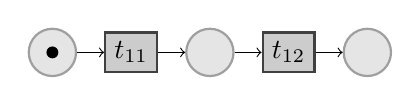
\begin{tikzpicture}
        \node at (0,0) [place,tokens=1] (a) {};
        \node at (1,0) [transition]     (b) {$t_{11}$};
        \node at (2,0) [place]          (c) {};
        \node at (3,0) [transition]     (d) {$t_{12}$};
        \node at (4,0) [place]          (e) {};

        \draw [->] (a) -- (b);
        \draw [->] (b) -- (c);
        \draw [->] (c) -- (d);
        \draw [->] (d) -- (e);
      \end{tikzpicture}
      \caption[The \emph{Causality} workflow primitive]{Causality}
      \label{figure-Causality}
    \end{center}
  \end{minipage}
  \hfill
  \begin{minipage}{0.45\textwidth}
    \begin{center}
      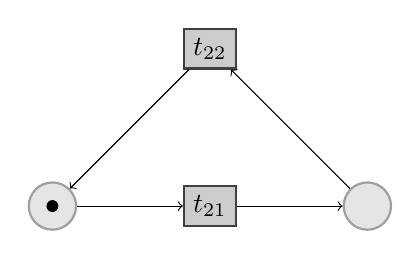
\begin{tikzpicture}
        \node at (0,0) [place,tokens=1] (a) {};
        \node at (2,0) [transition]     (b) {$t_{21}$};
        \node at (4,0) [place]          (c) {};
        \node at (2,2) [transition]     (d) {$t_{22}$};

        \draw [->] (a) -- (b);
        \draw [->] (b) -- (c);
        \draw [->] (c) -- (d);
        \draw [->] (d) -- (a);
      \end{tikzpicture}
      \caption[The \emph{Iteration} workflow primitive]{Iteration}
      \label{figure-Iteration}
    \end{center}
  \end{minipage}
\end{figure}

\begin{figure}[htb]
  \begin{minipage}{0.45\textwidth}
    \begin{center}
      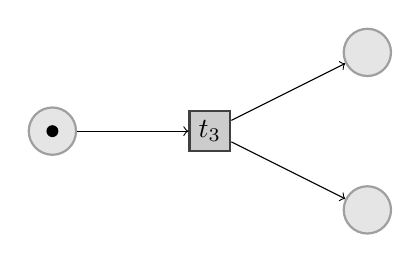
\begin{tikzpicture}
        \node at (0,1) [place,tokens=1] (a) {};
        \node at (2,1) [transition]     (b) {$t_{3}$};
        \node at (4,2) [place]          (c) {};
        \node at (4,0) [place]          (d) {};

        \draw [->] (a) -- (b);
        \draw [->] (b) -- (c);
        \draw [->] (b) -- (d);
      \end{tikzpicture}
      \caption[The \emph{AND-Split} workflow primitive]{AND-Split}
      \label{figure-ANDSplit}
    \end{center}
  \end{minipage}
  \hfill
  \begin{minipage}{0.45\textwidth}
    \begin{center}
      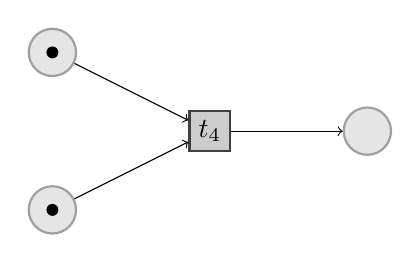
\begin{tikzpicture}
        \node at (0,2) [place,tokens=1] (a) {};
        \node at (0,0) [place,tokens=1] (b) {};
        \node at (2,1) [transition]     (c) {$t_{4}$};
        \node at (4,1) [place]          (d) {};

        \draw [->] (a) -- (c);
        \draw [->] (b) -- (c);
        \draw [->] (c) -- (d);
      \end{tikzpicture}
      \caption[The \emph{AND-Join} workflow primitive]{AND-Join}
      \label{figure-ANDJoin}
    \end{center}
  \end{minipage}
\end{figure}

\begin{figure}[htb]
  \begin{minipage}{0.45\textwidth}
    \begin{center}
      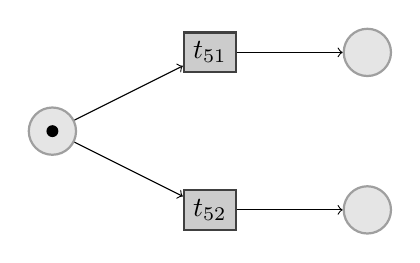
\begin{tikzpicture}
        \node at (0,1) [place,tokens=1] (a) {};
        \node at (2,2) [transition]     (b) {$t_{51}$};
        \node at (2,0) [transition]     (c) {$t_{52}$};
        \node at (4,2) [place]          (d) {};
        \node at (4,0) [place]          (e) {};

        \draw [->] (a) -- (b);
        \draw [->] (a) -- (c);
        \draw [->] (b) -- (d);
        \draw [->] (c) -- (e);
      \end{tikzpicture}
      \caption[The \emph{OR-Split} workflow primitive]{OR-Split}
      \label{figure-ORSplit}
    \end{center}
  \end{minipage}
  \hfill
  \begin{minipage}{0.45\textwidth}
    \begin{center}
      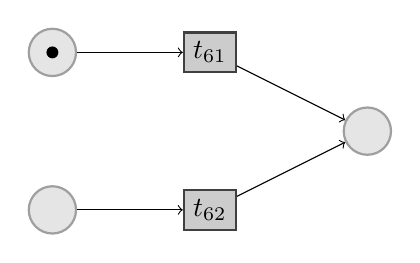
\begin{tikzpicture}
        \node at (0,2) [place,tokens=1] (a) {};
        \node at (0,0) [place]          (b) {};
        \node at (2,2) [transition]     (c) {$t_{61}$};
        \node at (2,0) [transition]     (d) {$t_{62}$};
        \node at (4,1) [place]          (e) {};

        \draw [->] (a) -- (c);
        \draw [->] (b) -- (d);
        \draw [->] (c) -- (e);
        \draw [->] (d) -- (e);
      \end{tikzpicture}
      \caption[The \emph{OR-Join} workflow primitive]{OR-Join}
      \label{figure-ORJoin}
    \end{center}
  \end{minipage}
\end{figure}

Finite Automata are another formalism that can be used to describe workflows \cite{ARK03}.

\section{Workflow Patterns}
\label{section-WorkflowPatterns}

In Chapter 3 of his PhD thesis \cite{BK03}, Kiepuszewski lists
\emph{requirements for workflow languages through workflow patterns}.

Much like the software design patterns \cite{GoF94}, these workflow patterns
describe recurring solutions to common problems. They are relevant to both the
implementor and the user of a workflow management system. The former uses the
workflow patterns as a common vocabulary for workflow description language
constructs and to define the semantics of a workflow model (see
Chapter~\ref{chapter-WorkflowModel}) whereas the latter uses them as a guide while
formulating his workflow in the workflow system's description language. The
workflow patterns also faciliate the comparison with other workflow systems
with regard to expressiveness and power.
 
In Chapter 4 of his PhD thesis \cite{BK03}, Kiepuszewski maps the workflow
patterns that he identified to Petri nets to provide a formal foundation for
this more pragmatic approach to defining workflow semantics.

In this section we discuss the subset of the workflow patterns identified by
Kiepuszewski that is directly supported by the software that has been
implemented as part of this thesis.

\subsection{Basic Control Flow Patterns}
\label{subsection-BasicControlFlowPatterns}

The workflow patterns for basic control flow \emph{capture elementary aspects
of process control} and \emph{closely match the definitions of elementary
control flow concepts provided by the Workflow Management Coalition in
\cite{WfMC95,WfMC99}}.

\subsubsection{Sequence}

The \emph{Sequence} workflow pattern represents linear execution of workflow
steps: one action of a workflow is activated unconditionally (for example
\emph{B} in Figure \ref{figure-Sequence}) after another (for example \emph{A}
in Figure \ref{figure-Sequence}) finished executing.

\begin{figure}[hbt]
\begin{center}
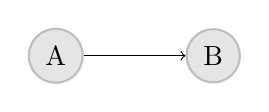
\begin{tikzpicture}
  \node at ( 0, 0) [node] (A) {A};
  \node at ( 2, 0) [node] (B) {B};
  \draw [->] (A) to (B);
\end{tikzpicture}
\end{center}
\caption[The \emph{Sequence} workflow pattern]{Sequence}
\label{figure-Sequence}
\end{figure}

\textbf{Use Case Example:} After an order is placed, the credit card specified by the
customer is charged. 

\subsubsection{Parallel Split (AND-Split)}

The \emph{Parallel Split} workflow pattern divides one thread of execution
(for example the one that activates \emph{A} in Figure
\ref{figure-ParallelSplit}) unconditionally into multiple parallel threads of
execution (for example the ones that start in \emph{B}, \emph{C}, and \emph{D}
in Figure \ref{figure-ParallelSplit}).

\begin{figure}[htb]
  \begin{minipage}{0.45\textwidth}
    \begin{center}
      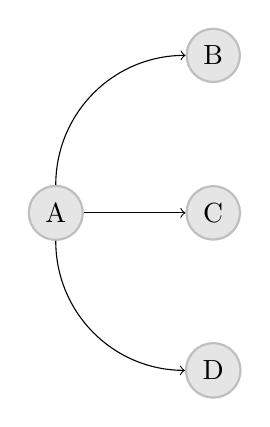
\begin{tikzpicture}
        \node at ( 0, 0) [node] (A) {A};
        \node at ( 2, 2) [node] (B) {B};
        \node at ( 2, 0) [node] (C) {C};
        \node at ( 2,-2) [node] (D) {D};
        \draw [->,bend left=45] (A) to (B);
        \draw [->] (A) to (C);
        \draw [->,bend right=45] (A) to (D);
      \end{tikzpicture}
      \caption[The \emph{Parallel Split} workflow pattern]{Parallel Split}
      \label{figure-ParallelSplit}
    \end{center}
  \end{minipage}
  \hfill
  \begin{minipage}{0.45\textwidth}
    \begin{center}
      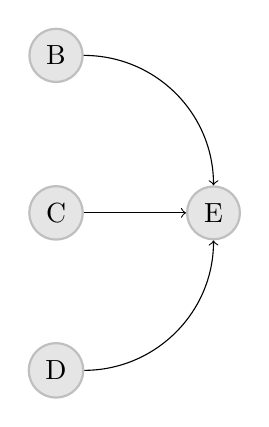
\begin{tikzpicture}
        \node at ( 0, 2) [node] (B) {B};
        \node at ( 0, 0) [node] (C) {C};
        \node at ( 0,-2) [node] (D) {D};
        \node at ( 2, 0) [node] (E) {E};
        \draw [->,bend left=45] (B) to (E);
        \draw [->] (C) to (E);
        \draw [->,bend right=45] (D) to (E);
      \end{tikzpicture}
      \caption[The \emph{Synchronization} workflow pattern]{Synchronization}
      \label{figure-Synchronization}
    \end{center}
  \end{minipage}
\end{figure}

\textbf{Use Case Example:} After the credit card specified by the customer has been
successfully charged, the activities of sending a confirmation email and
starting the shipping process can be executed in parallel.

\subsubsection{Synchronization (AND-Join)}

The \emph{Synchronization} workflow pattern synchronizes multiple parallel
threads of execution (for example the ones that end in \emph{B}, \emph{C},
and \emph{D} in Figure \ref{figure-Synchronization}) into a single thread of
execution (for example the one that starts in \emph{E} in Figure
\ref{figure-Synchronization}).

Workflow execution continues once all threads of execution that are to be
synchronized have finished executing (exactly once).

\textbf{Use Case Example:} After the confirmation email has been sent and
the shipping process has been completed, the order can be archived.

The workflow patterns that have been discussed so far handle the
\emph{unconditional routing} of control flow. We will now take a look at the
workflow patterns for \emph{conditional routing}.

\subsubsection{Exclusive Choice (XOR-Split)}

The \emph{Exclusive Choice} workflow pattern defines multiple possible paths
(for example the ones that start in \emph{B}, \emph{C}, and \emph{D} in Figure
\ref{figure-ExclusiveChoice}) for the workflow of which exactly one is chosen
(for example the one that starts in \emph{C} in Figure
\ref{figure-ExclusiveChoice}).

\begin{figure}[htb]
  \begin{minipage}{0.45\textwidth}
    \begin{center}
      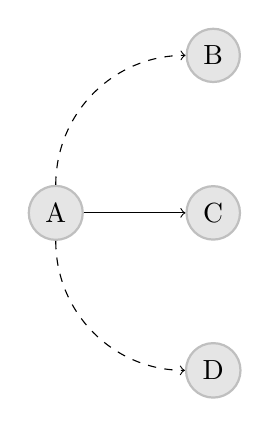
\begin{tikzpicture}
        \node at ( 0, 0) [node] (A) {A};
        \node at ( 2, 2) [node] (B) {B};
        \node at ( 2, 0) [node] (C) {C};
        \node at ( 2,-2) [node] (D) {D};
        \draw[dashed] [->,bend left=45] (A) to (B);
        \draw [->] (A) to (C);
        \draw[dashed] [->,bend right=45] (A) to (D);
      \end{tikzpicture}
      \caption[The \emph{Exclusive Choice} workflow pattern]{Exclusive Choice}
      \label{figure-ExclusiveChoice}
    \end{center}
  \end{minipage}
  \hfill
  \begin{minipage}{0.45\textwidth}
    \begin{center}
      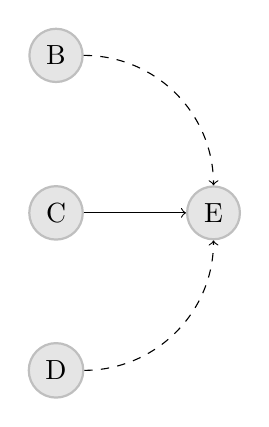
\begin{tikzpicture}
        \node at ( 0, 2) [node] (B) {B};
        \node at ( 0, 0) [node] (C) {C};
        \node at ( 0,-2) [node] (D) {D};
        \node at ( 2, 0) [node] (E) {E};
        \draw[dashed] [->,bend left=45] (B) to (E);
        \draw [->] (C) to (E);
        \draw[dashed] [->,bend right=45] (D) to (E);
      \end{tikzpicture}
      \caption[The \emph{Simple Merge} workflow pattern]{Simple Merge}
      \label{figure-SimpleMerge}
    \end{center}
  \end{minipage}
\end{figure}

\textbf{Use Case Example:} After an order has been received, the payment can
be performed by credit card or bank transfer.

\subsubsection{Simple Merge (XOR-Join)}

The \emph{Simple Merge} workflow pattern is to be used to merge the possible
paths that are defined by a preceding \emph{Exclusive Choice}. It is assumed
that of these possible paths exactly one is taken (for example \emph{C} in
Figure \ref{figure-SimpleMerge}) and no synchronization takes place.

\textbf{Use Case Example:} After the payment has been performed by either
credit card or bank transfer, the order can be processed further.

\subsection{Advanced Branching and Synchronization}
\label{subsection-AdvancedBranchingAndSynchronization}

The workflow patterns for advanced branching and synchronization \emph{do
not have straightforward support in most [of the] workflow engines [that
Kiepuszewski evaluated]} (see Table~\ref{table-ComparisonWorkflowSystems}).
\emph{Nevertheless, they are quite common in real-life business scenarios}.

\subsubsection{Multi-Choice (OR-Split)}

The \emph{Multi-Choice} workflow pattern defines multiple possible paths
(for example the ones that start in \emph{B}, \emph{C}, and \emph{D} in Figure
\ref{figure-MultiChoice}) for the workflow of which one or more are chosen
(for example the ones that start in \emph{B} and \emph{D} in Figure
\ref{figure-MultiChoice}). It is a generalization of the Parallel Split and
Exclusive Choice workflow patterns.

\begin{figure}[htb]
  \begin{minipage}{0.45\textwidth}
    \begin{center}
      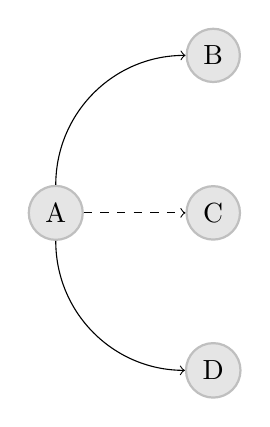
\begin{tikzpicture}
        \node at ( 0, 0) [node] (A) {A};
        \node at ( 2, 2) [node] (B) {B};
        \node at ( 2, 0) [node] (C) {C};
        \node at ( 2,-2) [node] (D) {D};
        \draw [->,bend left=45] (A) to (B);
        \draw[dashed] [->] (A) to (C);
        \draw [->,bend right=45] (A) to (D);
      \end{tikzpicture}
      \caption[The \emph{Multi-Choice} workflow pattern]{Multi-Choice}
      \label{figure-MultiChoice}
    \end{center}
  \end{minipage}
  \hfill
  \begin{minipage}{0.45\textwidth}
    \begin{center}
      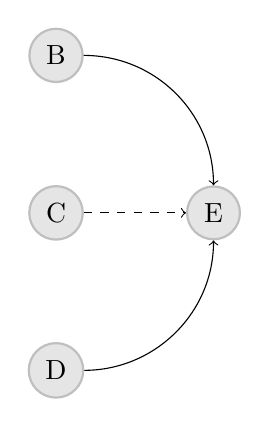
\begin{tikzpicture}
        \node at ( 0, 2) [node] (B) {B};
        \node at ( 0, 0) [node] (C) {C};
        \node at ( 0,-2) [node] (D) {D};
        \node at ( 2, 0) [node] (E) {E};
        \draw [->,bend left=45] (B) to (E);
        \draw[dashed] [->] (C) to (E);
        \draw [->,bend right=45] (D) to (E);
      \end{tikzpicture}
      \caption[The \emph{Synchronizing Merge} workflow pattern]{Synchronizing Merge}
      \label{figure-SynchronizingMerge}
    \end{center}
  \end{minipage}
\end{figure}

\subsubsection{Synchronizing Merge}

The \emph{Synchronizing Merge} workflow pattern is to be used to synchronize
multiple parallel threads of execution that are activated by a preceding
\emph{Multi-Choice} (for example the ones that end in \emph{B} and \emph{D}
in Figure \ref{figure-SynchronizingMerge}).

\subsubsection{Discriminator}

The \emph{Discriminator} workflow pattern can be applied when the assumption
we made for the \emph{Simple Merge} workflow pattern does not hold. It can
deal with merge situations where multiple incoming branches may run in
parallel.

It activates its outgoing node after being activated by the first incoming
branch and then waits for all remaining branches to complete before it resets
itself. After the reset the \emph{Discriminator} can be triggered again.

\textbf{Use Case Example:} To improve response time, an action is delegated to
several distributed servers. The first response proceeds the flow, the other
responses are ignored.

\subsection{Structural Patterns}
\label{subsection-StructuralPatterns}

The structural workflow patterns deal with restrictions that different workflow
models can impose.

\subsubsection{Arbitrary Cycles}

A common restriction workflow models impose is that arbitrary cycles, ie. one
or more activities are done repeatedly, are not supported. As an alternative,
special loop constructs that mark the start and end point of a structured cycle
are offered.

\subsubsection{Implicit Termination}

The execution of the workflow is (successfully) terminated when there are no
activated activities left and no other activity can be activated. This implicit
termination of workflow execution can be used in addition to explicit end
activities.

\subsection{Cancellation Patterns}
\label{subsection-CancellationPatterns}

\subsubsection{Cancel Case}

The execution of a workflow instance is cancelled.

\textbf{Use Case Example:} An order is cancelled.

\section{Summary}

This chapter presented Petri nets as a general, well understood and well
researched, theory for concurrency and the workflow patterns as an pragmatic
approach to describe the semantics of workflow routing constructs.

We will use the workflow patterns in Chapter~\ref{chapter-Requirements} during
the requirements analysis and in Chapter~\ref{chapter-WorkflowModel} to define
the semantics of the workflow model for the software that has been developed as
part of this thesis.

\chapter{Technology}
\label{chapter-Technology}

This chapter gives an introduction to the technology stack (PHP, eZ~Publish,
eZ~Components) that is relevant to and used by the software that has been
implemented as part of this thesis.

\section{PHP}

PHP is a widely-used scripting language. Initially designed for Web
programming, it has matured to a general-purpose programming language that
supports both procedural and object-oriented programming. PHP makes strong
inroads into large-scale, business-critical Web systems. For instance,
financial institutions develop and maintain BASEL II credit and insurance
rating tools using PHP and Yahoo! runs all its business on PHP (except the core
of the search engine). As of version 5, released July 2004, the PHP language
features an object model that is similar to the ones of Java and C\# and
integrates ideas from other programming languages. The key technical
contributor to PHP's success is its sim\-pli\-city, which translates into
shorter development cycles, easier maintenance, and lower training costs. The
second one is social -- the very large and vibrant community around it, which
develops not only PHP itself but also thousands of open source applications
that can be used off-the-shelf or as references for new applications.

\cite{SB05} gives an introduction to object-oriented programming with PHP 5.

\section{eZ Publish}
\label{section-eZPublish}

eZ~Publish is the Enterprise Content Management System developed by
eZ~Systems~AS. With its framework architechture, it is both an
out-of-the-box solution as well as a platform that can be customized and
extended to suit the specific requirements of a customer.

Figure~\ref{figure-ArchitectureEZPublish3} shows an overview of the
architecture of eZ~Publish in its current version.

\begin{figure}[hbt]
\begin{center}
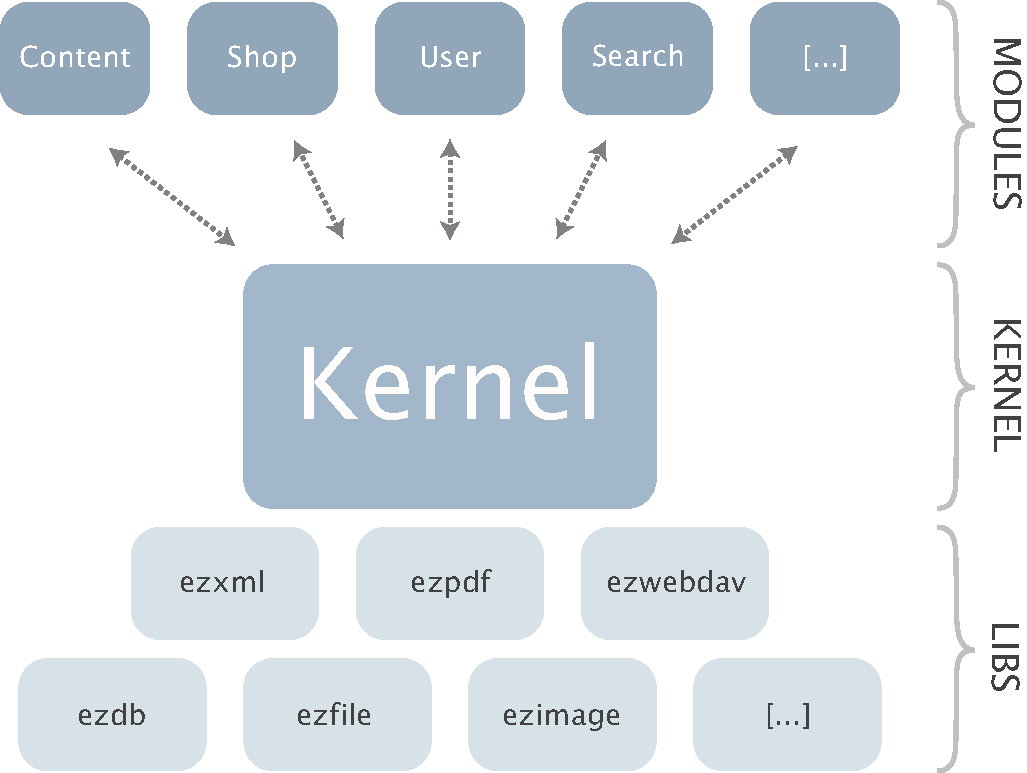
\includegraphics[width=10cm]{figures/ArchitectureEZPublish3}\\[5mm]
\end{center}
\caption{The Architecture of eZ Publish 3}
\label{figure-ArchitectureEZPublish3}
\end{figure}

The \emph{libraries} are the main building blocks of the system and are
designed as reuseable general purpose PHP classes. Although they are not
dependant on other parts of the system, some of them are not usable outside
the scope of eZ~Publish as the functionality they provide is tightly
coupled to eZ~Publish.

The \emph{kernel} makes up the system's core and is responsible, among other
things, for content handling and versioning, access control, and workflows. 

Whereas the kernel and the libraries provide rather low-level functionality,
the \emph{modules} implement the higher-level functionality of the system. They
provide web-based interfaces to functionality that is, for instance, part of
the kernel. For example, the content module provides an interface that makes
it possible to use a web browser to manage content. A module consists of two
components: at least one \emph{view} and one or more optional
\emph{fetch functions}. The former implement the actual web interface of the
module. The latter allow for the extraction of data through a module from
within a \emph{template}.

eZ~Publish uses an object-oriented approach to organize and store content
and allows for the creation of custom structures that fit the needs of the
customer. The system offers a selection of fundamental building blocks and
mechanisms that together provide a flexible content management solution. An
actual data structure is described using something called a \emph{content class}.
A content class is built up of attributes. An \emph{attribute} can be thought of
as a field, for example the ''title'' field in a structure designed to store
news articles. The description of the entire structure would be refferred to as
the ''article class''. The characteristics of an attribute inside the class are
determined by the \emph{datatype} that was chosen to represent that attribute.

\begin{figure}[hbt]
\begin{center}
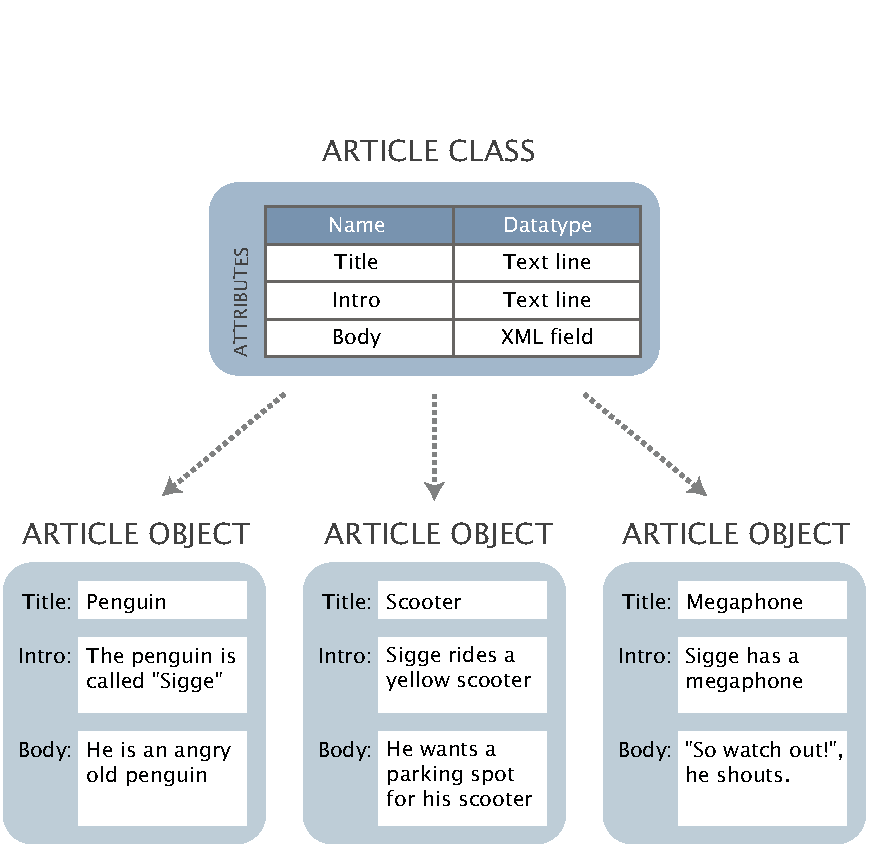
\includegraphics[width=10cm]{figures/ContentObject}\\[5mm]
\end{center}
\caption{The \emph{Content Object} abstraction of eZ Publish}
\label{figure-ContentObject}
\end{figure}

A \emph{content object} is an instance of a content class. While the class
only defines the data structure, it is the content objects themselves that
contain actual data. Once a content class is defined, several instances of
that class can be created. Figure \ref{figure-ContentObject} illustrates
this relationship of datatypes, attributes, content classes, and objects.

\section{eZ Components}
\label{section-eZComponents}

As part of the development on eZ~Publish Telemark, the next major version
of its eZ~Publish Enterprise Content Management System software, eZ~Systems~AS
has begun refactoring of core functionality from eZ~Publish itself into a
library of reusable PHP components that provide low-level functionality such
as database abstraction, object persistence and caching. This library is
called eZ~Components.

Figure \ref{figure-eZComponents} shows an overview of the eZ~Components
library. One of the design goals of the library is to minimize the number of
dependencies between its various components. A component may only depend on
the \texttt{Base} component. Optional dependencies are handled through
so-called \emph{tie-in} components that tie two components together.

\begin{figure}[hbt]
\begin{center}
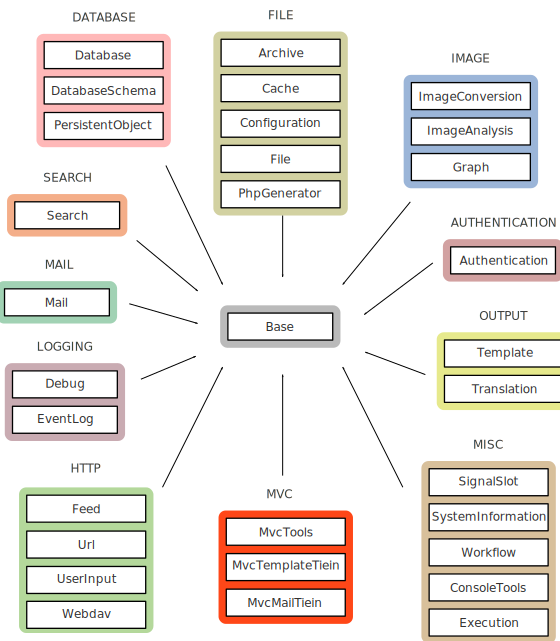
\includegraphics[width=10cm]{figures/ezcomponents}\\[5mm]
\end{center}
\caption{The eZ Components library for PHP 5.}
\label{figure-eZComponents}
\end{figure}

The workflow engine that has been developed as part of this thesis is
released under the New BSD License as part of the eZ~Components library and
utilizes the \texttt{Database} and \texttt{DatabaseSchema} components for
database abstraction and the \texttt{EventLog} component for logging
abstraction.

\chapter{Requirements}
\label{chapter-Requirements}

This chapter is divided into two sections.
Section \ref{section-RequirementseZPublish3} presents the workflow mechanism
that is part of eZ~Publish~3, the current version of the Enterprise Content
Management System by eZ~Systems~AS. Section \ref{section-RequirementseZPublishTelemark}
discusses the requirements that the workflow engine for eZ~Publish~Telemark,
the next version of eZ~Publish, needs to fulfill.

\section{eZ Publish 3}
\label{section-RequirementseZPublish3}

eZ~Publish~3 comes with an integrated workflow mechanism that makes it
possible to perform different tasks with or without user interaction.

\begin{figure}[hbt]
\begin{center}
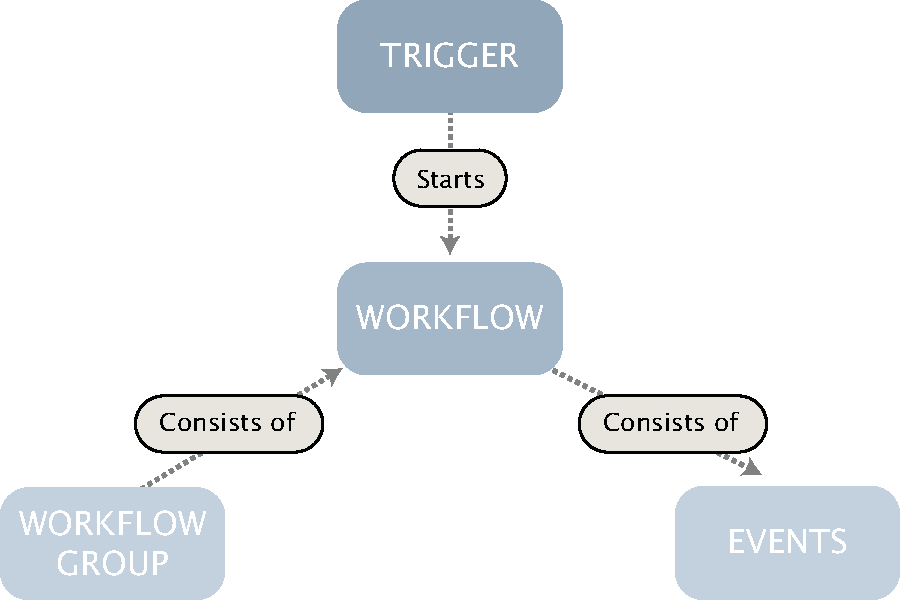
\includegraphics[width=10cm]{figures/WorkflowEZPublish3}\\[5mm]
\end{center}
\caption{The workflow system in eZ Publish 3}
\label{figure-WorkflowEZPublish3}
\end{figure}

Figure~\ref{figure-WorkflowEZPublish3} shows the components that comprise this
mechanism.

An \emph{event} performs a specific task. eZ~Publish~3 ships with a library
of events and custom events can be implemented in PHP.

A \emph{workflow} defines an ordered sequence in which workflow events are
executed and is initiated by a \emph{trigger} that is associated with a
function of a module (see Section~\ref{section-eZPublish}). It will start the
specified workflow either before or after that function has finished
executing.

\begin{figure}[hbt]
\begin{center}
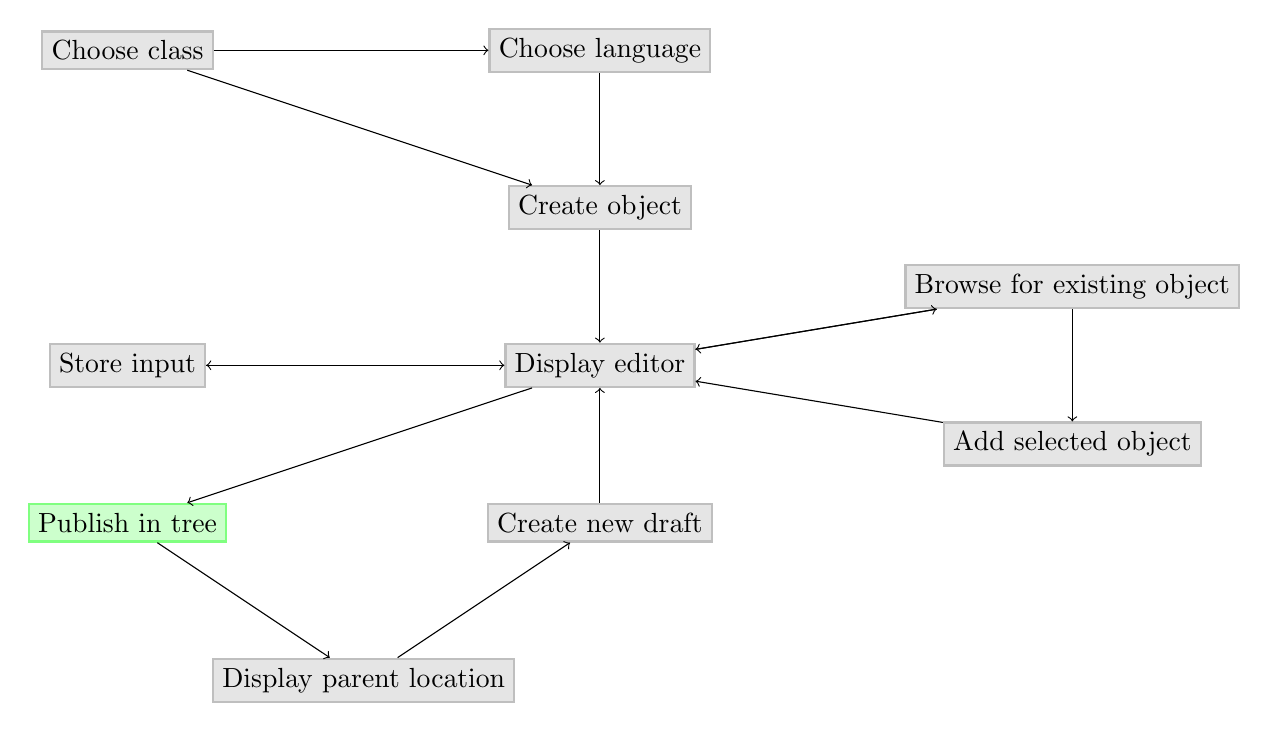
\begin{tikzpicture}
  \node at (-6, 4) [activity] (ChooseClass) {Choose class};
  \node at ( 0, 4) [activity] (ChooseLanguage) {Choose language};
  \node at ( 0, 2) [activity] (CreateObject) {Create object};
  \node at (-6, 0) [activity] (StoreInput) {Store input};
  \node at ( 0, 0) [activity] (DisplayEditor) {Display editor};
  \node at ( 6, 1) [activity] (Browse) {Browse for existing object};
  \node at ( 6,-1) [activity] (Add) {Add selected object};
  \node at ( 0,-2) [activity] (CreateDraft) {Create new draft};
  \node [rectangle,draw=green!50,fill=green!20,thick] at (-6,-2) (Publish) {Publish in tree};
  \node at (-3,-4) [activity] (DisplayParent) {Display parent location};
  \draw [->] (ChooseClass) to (ChooseLanguage);
  \draw [->] (ChooseClass) to (CreateObject);
  \draw [->] (ChooseLanguage) to (CreateObject);
  \draw [->] (CreateObject) to (DisplayEditor);
  \draw [->] (DisplayEditor) to (StoreInput);
  \draw [->] (StoreInput) to (DisplayEditor);
  \draw [->] (Browse) to (DisplayEditor);
  \draw [->] (DisplayEditor) to (Browse);
  \draw [->] (Browse) to (Add);
  \draw [->] (Add) to (DisplayEditor);
  \draw [->] (CreateDraft) to (DisplayEditor);
  \draw [->] (DisplayEditor) to (Publish);
  \draw [->] (Publish) to (DisplayParent);
  \draw [->] (DisplayParent) to (CreateDraft);
\end{tikzpicture}
\end{center}
\caption{Workflow for publishing a content object in eZ Publish 3}
\label{figure-PublishObjectWorkflow}
\end{figure}

Figure \ref{figure-PublishObjectWorkflow} shows the built-in workflow for
publishing acontent object in eZ~Publish~3. This workflow can only be
customized at the \emph{Publish in tree} activity. This activity serves as the
trigger for a custom workflow that can be executed either before or after the
activity was executed.

\section{eZ Publish Telemark}
\label{section-RequirementseZPublishTelemark}

Both the architecture of the current eZ~Publish version as well as its
workflow feature have shortcomings that are to be overcome:

\begin{itemize}
\item Only some operations are workflows. This inconsistency has a negative
      effect on the maintainability of the software as a whole.
\item It is not easy to configure (hook in) the (internal) workflows. This
      makes extending the software hard.
\item Support for checking the state of executing workflows and control
      over them is limited.
\item Support for conditions is limited.
\end{itemize}

Eventually, the workflow component should become an important part of the
overall solution. However, it must not be tightly integrated or too much
dependent on other parts of the system (and vice versa). This means that
the workflow component must be flexible and provide good interfaces which
allow it to co-exist and plug into the software.

Georgakopoulos et. al. list general requirements for workflow management
systems:

\begin{quote}
\emph{To effectively support [workflow management], organizations must evolve
their existing computing environments to a new distributed environment that:
is \emph{component-oriented}, i.e. supports integration and interoperability
among loosely-coupled components [...], supports \emph{workflow applications}
corresponding to business or information process implementations [...],
ensures the correctness and reliability of applications in the presence of
concurrency and failures, and supports the evolution, replacement, and
addition of workflow applications and component systems as processes are
reengineered} \cite{DG95}.
\end{quote}

Following are the requirements set up by eZ~Systems~AS. We start with the
requirements that are relevant to the underlying workflow model of the
workflow component that is to be implemented:

\begin{itemize}
\item The workflow component should provide good support for expressing
      control flow using the workflow patterns (see
      Chapter~\ref{chapter-WorkflowModel}).
\item Any non-trivial operation in eZ~Publish, for instance the publishing,
      removal, and modification of content objects, should be a expressable
      through workflows.
\item Workflows should be composable through a concept of sub-workflows.
\end{itemize}

Now we come to the requirements that relate to the actual software
implementation:

\begin{itemize}
\item The workflow component has to be implemented using version 5 of the
      PHP programming language.
\item It should be possible to integrate workflows with the background
      processes of eZ~Publish (run workflow as background process, interact
      with a background process).
\item The workflow component should be customizable and extendable.
\item The data storage (for workflow schemas and the persistence of
      workflow instances) should be abstracted, relational databases must
      be supported as one backend.
\item Versioning of workflow schemas should be supported.
\item It should be possible to get information on the workflow instances
      that are currently executing.
\item It should be possible to manually control the workflow instances
      that are currently executing.
\item Simulation of workflow execution for debugging and testing purposes
      should be possible.
\end{itemize}

\subsection{Use Cases}

Here are two use cases that should be supported by the workflow engine
component that is to be implemented for eZ~publish Telemark as part of this
thesis. They are currently implemented using custom extensions for
eZ~publish~3.

\subsubsection{Multiple Approval, ISO Certification}

This scenario is from a current customer of the eZ~Publish ECMS providing
quality assurance for dairy products. The customer has information about
the dairy products stored in eZ~Publish. When they update any content
there is a strict ISO-governed process to follow. This process basically
consists of a \emph{five-level approval}:

\begin{itemize}
\item Bertrand produces an article.
\item Approver Level 1: B�rd decides who the next four approvers are.\\
      He can also edit the article and send it back to its creator.
\item Approver Level 2: Melissa reviews the article for political
      correctness.\\
      She can edit the article and send it back one level.
\item Approver Level 3: Vidar reviews the article for sales arguments.\\
      He can edit the article and and send it back one level.
\item Approver Level 4: Jennifer does grammar checks on the article.\\
      She can edit the article and and send it back one level.
\item Publisher: Markus approves the final article and chooses the time
      and location for publication.
\end{itemize}

\begin{figure}[hbt]
\begin{center}
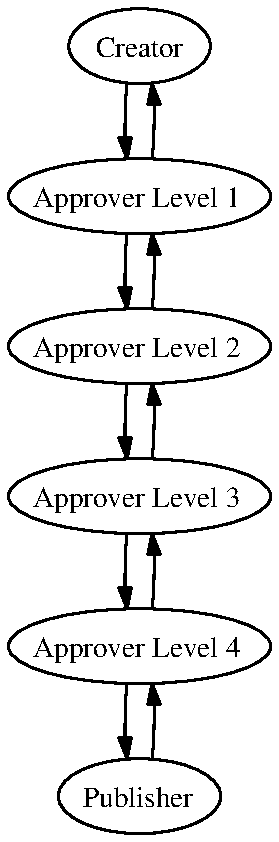
\includegraphics[height=10cm]{figures/MultipleApproval}\\[5mm]
\end{center}
\caption{The \emph{Multiple Approval} workflow}
\label{figure-MultipleApproval}
\end{figure}

It is possible to see all on-going processes for an administrator. He or
she can see each article as well as its state and which person currently
handles it.

\subsubsection{Employment Process}

This scenario is from the intranet of a current customer of the eZ~Publish
ECMS and is used when a new employee is hired.

\begin{itemize}
\item One person creates an Employee object (including name, address,
      email, etc.).
\item An e-mail with a link for final approval of the employment is
      sent to the CEO.
\item Once the CEO has approved the new employment three parallel
      activities are started:
      \begin{itemize}
      \item An e-mail to the system administrator is sent with the
            request to create e-mail and other accounts.\\
            The e-mail contains a link for the system administrator to
            click when he is done.
      \item An automatic process is started to set up accounts on
            different systems.
      \item An e-mail to the administration is sent with the request
            to buy new hardware for the new employee.
      \end{itemize}
\item Once these three activities have been completed, the workflow
      continues.
\item The Employee object is published.
\item An e-mail with detailed information is sent to the new employee.
\end{itemize}

\begin{figure}[hbt]
\begin{center}
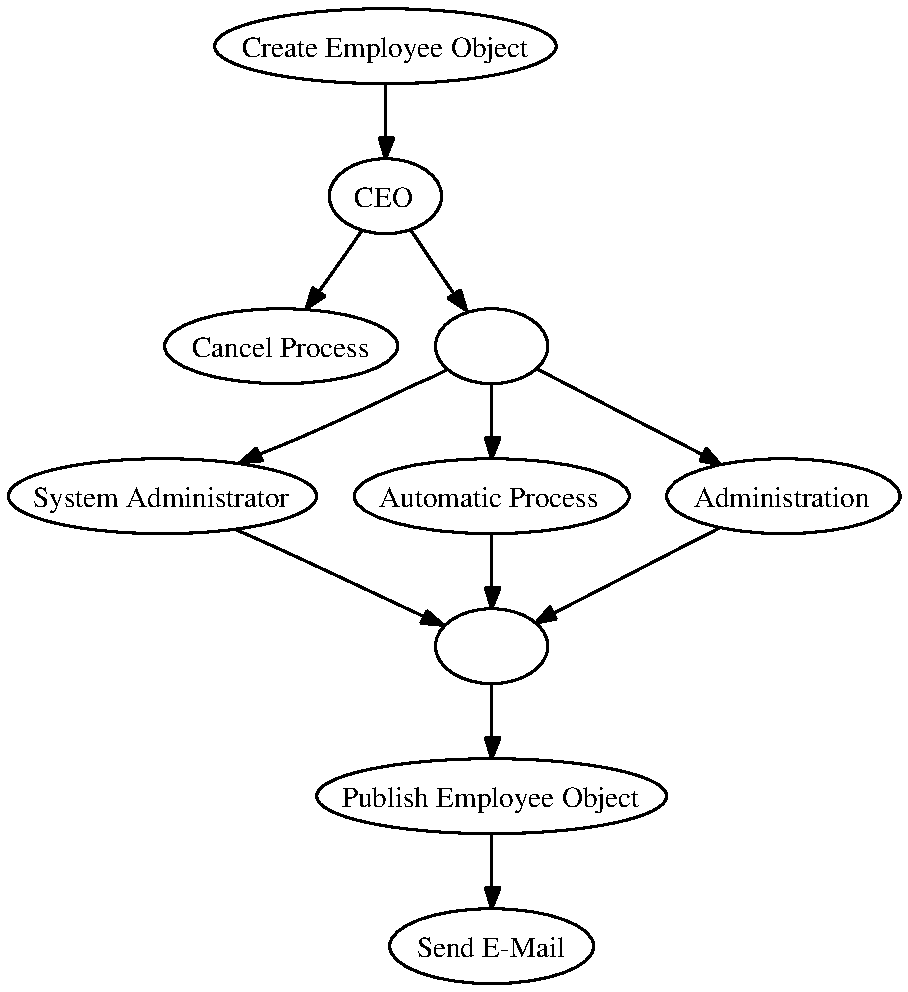
\includegraphics[height=10cm]{figures/EmploymentProcess}\\[5mm]
\end{center}
\caption{The \emph{Employment Process} workflow}
\label{figure-EmploymentProcess}
\end{figure}

The on-going status for all employment processes at any time is available
to anyone with the appropriate permissions.

\section{Summary}

This chapter discussed the requirements for the software that has been
developed as part of this thesis. This software will replace the workflow
engine of eZ~Publish~3 which has severe limitations with regard to the
underlying workflow model (only one directly supported workflow pattern)
and the software implementation (not easily extendable).

\chapter{Workflow Model}
\label{chapter-WorkflowModel}

This chapter presents the semantics and syntax of the workflow model that is
the foundation for the software that has been developed as part of this thesis.

\section{Semantics}

\subsection{Activities and Transitions}

The workflow model is activity-based. The activities that are to be completed
throughout the workflow and the transitions between them are mapped to the
nodes and edges of a directed graph. This choice was made to faciliate the
application of the Graph-Oriented Programming paradigm for the implementation
of the software component that is discussed in
Chapter~\ref{chapter-DesignAndImplementation}. Using a directed graph as the
foundation for the workflow model makes it possible to define the syntax of
the workflow description language using the formalism of graph grammars (see
Section~\ref{section-Syntax}).

\subsubsection{Graph Traversal and Execution Strategy}

The execution of a workflow starts with the graph's only \emph{Start} node. A
graph may have one or more \emph{End} nodes that explicitly terminate the
workflow execution.

After a node has finished executing, it can activate one or more of its
possible outgoing nodes. Activation adds a node to a set of nodes that
are waiting for execution. During each execution step, a node from this set
is executed. When the execution of a node has been completed, the node is
removed from the set.

The workflow execution is implicitly terminated when no nodes are activated
and no more nodes can be activated (see the \emph{Implicit Termination}
workflow pattern from \cite{BK03} that was discussed in Section
\ref{section-WorkflowPatterns}).

\subsection{State and Workflow Variables}

The workflow model supports state through the concept of workflow variables.
Such a variable can either be requested as user input (from an \emph{Input}
node) or be set and manipulated through the \emph{VariableSet},
\emph{VariableAdd}, \emph{VariableSub}, \emph{VariableMul}, \emph{VariableDiv},
\emph{VariableIncrement}, and \emph{VariableDecrement} nodes.

While a \emph{VariableSet} node may set the value of a workflow variable to
any type that is supported by the underlying programming language, the other
variable manipulation nodes only operate on numbers.

Variables are bound to the scope of the thread in which they were defined.
This allows parallel threads of execution to use variables of the same name
without side effects.

\subsubsection{Wait States}

When the execution of a workflow reaches an \emph{Input} node (see above),
the execution is suspended until such time when the user input has been
provided and the execution can be resumed.

\subsection{Control Flow}

The control flow semantics of the workflow model draws upon the workflow
patterns from \cite{BK03} that were discussed in Section
\ref{section-WorkflowPatterns}. The \emph{Sequence}, \emph{Parallel Split},
\emph{Synchronization}, \emph{Exclusive Choice}, \emph{Simple Merge},
\emph{Multi-Choice}, \emph{Synchronizing Merge}, and \emph{Discriminator}
workflow patterns are all directly supported by the workflow model.

\emph{Exclusive Choice} and \emph{Multi-Choice} nodes have branching
conditions attached to them that operate on workflow variables to make their
control flow decisions.

\subsection{Action Nodes and Service Objects}

So far we have only discussed nodes that control the flow and that can
manipulate workflow variables. We are still missing a type of nodes that
actually performs an activity. This is where the \emph{Action} node comes
into play.

When the execution of a workflow reaches an \emph{Action} node, the
business logic of the attached \emph{service object} is executed. Service
Objects ''live'' in the domain of the application into which the workflow
engine is embedded. They have read and write access to the workflow variables
to interact with the rest of the workflow.

\subsection{Sub-Workflows}

The workflow model supports sub-workflows to break down a complex workflow
into parts that are easier to conceive, understand, maintain, and which can
be reused.

A sub-workflow is started when the respective \emph{Sub-Workflow} node is
reached during workflow execution. The execution of the parent workflow is
suspended while the sub-workflow is executing. It is resumed once the
execution of the sub-workflow has ended.

\section{Syntax}
\label{section-Syntax}

\subsection{Graph Structure}

Graph Grammars are a formalism for the specification of visual languages. In
the following, we will use the \emph{reserved graph grammar} variant presented
by Zhang et al. in \cite{DQZ01}. It \emph{allows left-hand and right-hand
graphs of a production to have an arbitrary number of nodes and edges}. This
feature makes the graph grammars more expressive. A node in these graphs is a
two-level structure: a so-called \emph{super vertex} contains named vertices,
\emph{T (top)}, \emph{B (bottom)}, \emph{L (left)}, \emph{R (right)}. The
names correspond to the position of the vertex in the super vertex.

Figures \ref{figure-grammar-Axiom} to \ref{figure-grammar-Discriminator} show
the graph rewriting rules (productions) that make up the grammar for our
workflow model.

The \emph{Axiom} grammar rule shown in Figure~\ref{figure-grammar-Axiom}
expresses that an empty graph (left-hand side) can be transformed into a
graph that contains three nodes: a \emph{Start} node that has a
\emph{Statement} node as its only outgoing node, which in turn has an
\emph{End} node as its only outgoing node.

The \emph{Reduction} grammar rule shown in
Figure~\ref{figure-grammar-Reduction} expresses that a \emph{Statement} node
can be added to another \emph{Statement} node.

\begin{figure}[htb]
  \begin{minipage}{0.45\textwidth}
    \begin{center}
      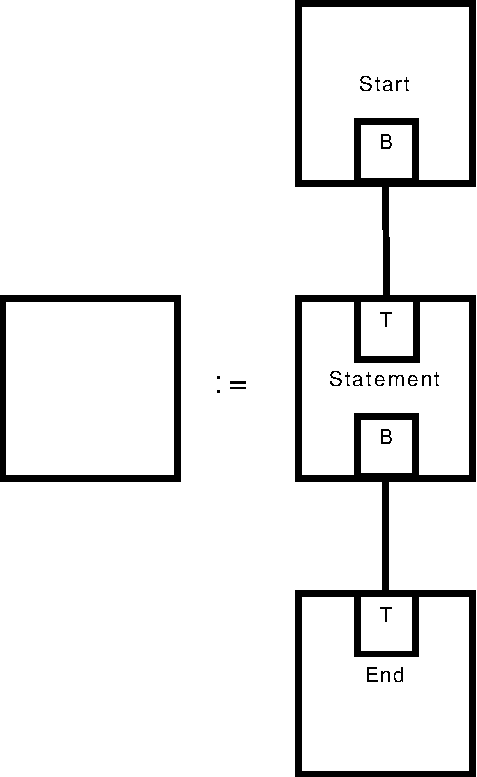
\includegraphics[width=4cm]{figures/grammar/axiom}\\[5mm]
      \caption[The \emph{Axiom} grammar rule]{Axiom}
      \label{figure-grammar-Axiom}
    \end{center}
  \end{minipage}
  \hfill
  \begin{minipage}{0.45\textwidth}
    \begin{center}
      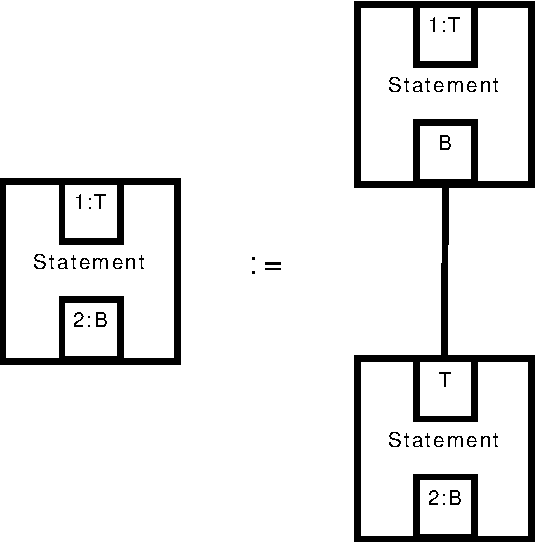
\includegraphics[width=4cm]{figures/grammar/reduction}\\[5mm]
      \caption[The \emph{Reduction} grammar rule]{Reduction}
      \label{figure-grammar-Reduction}
    \end{center}
  \end{minipage}
\end{figure}

\begin{figure}[htb]
  \begin{minipage}{0.45\textwidth}
    \begin{center}
      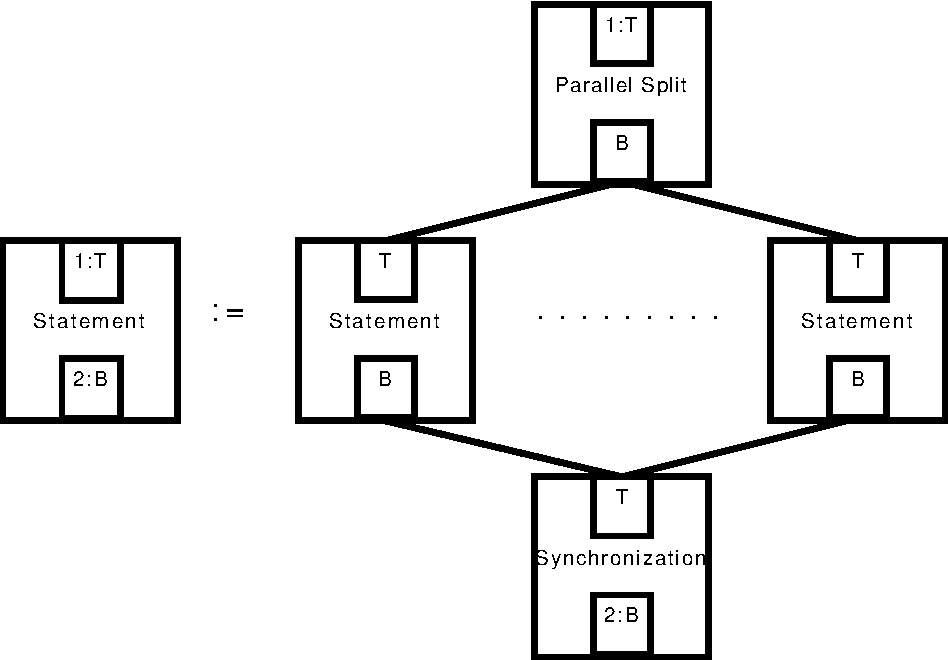
\includegraphics[width=7cm]{figures/grammar/and}\\[5mm]
      \caption[The \emph{AND} grammar rule]{AND}
      \label{figure-grammar-AND}
    \end{center}
  \end{minipage}
  \hfill
  \begin{minipage}{0.45\textwidth}
    \begin{center}
      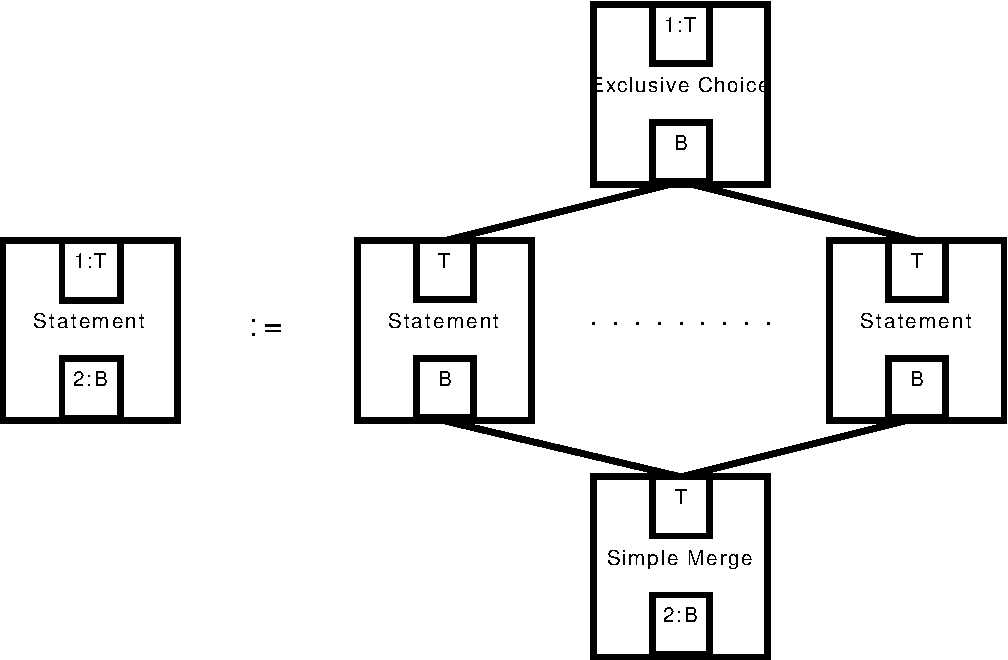
\includegraphics[width=7cm]{figures/grammar/xor}\\[5mm]
      \caption[The \emph{XOR} grammar rule]{XOR}
      \label{figure-grammar-XOR}
    \end{center}
  \end{minipage}
\end{figure}

A \emph{Statement} node can either be replaced by applying the grammar rules
shown in Figure~\ref{figure-grammar-AND} to \ref{figure-grammar-Discriminator}
or by replacing it with a node of type \emph{Action}, \emph{End}, \emph{Input},
\emph{Sub-Workflow}, \emph{VariableSet}, \emph{VariableAdd}, \emph{VariableSub},
\emph{VariableMul}, \emph{VariableDiv}, \emph{VariableIncrement}, and
\emph{VariableDecrement}.

\begin{figure}[htb]
  \begin{minipage}{0.45\textwidth}
    \begin{center}
      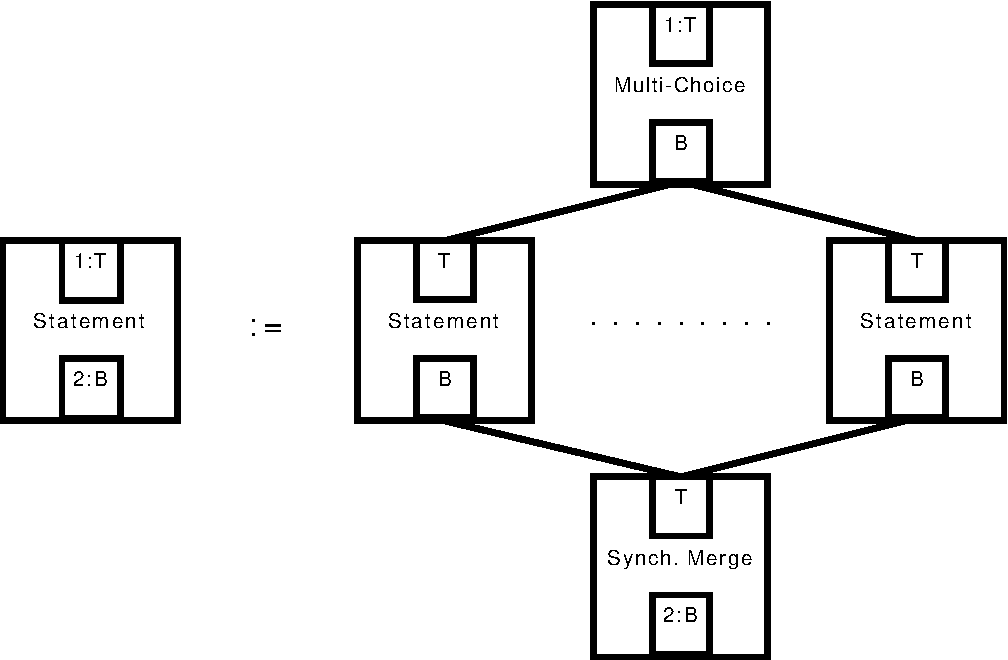
\includegraphics[width=7cm]{figures/grammar/or}\\[5mm]
      \caption[The \emph{OR} grammar rule]{OR}
      \label{figure-grammar-OR}
    \end{center}
  \end{minipage}
  \hfill
  \begin{minipage}{0.45\textwidth}
    \begin{center}
      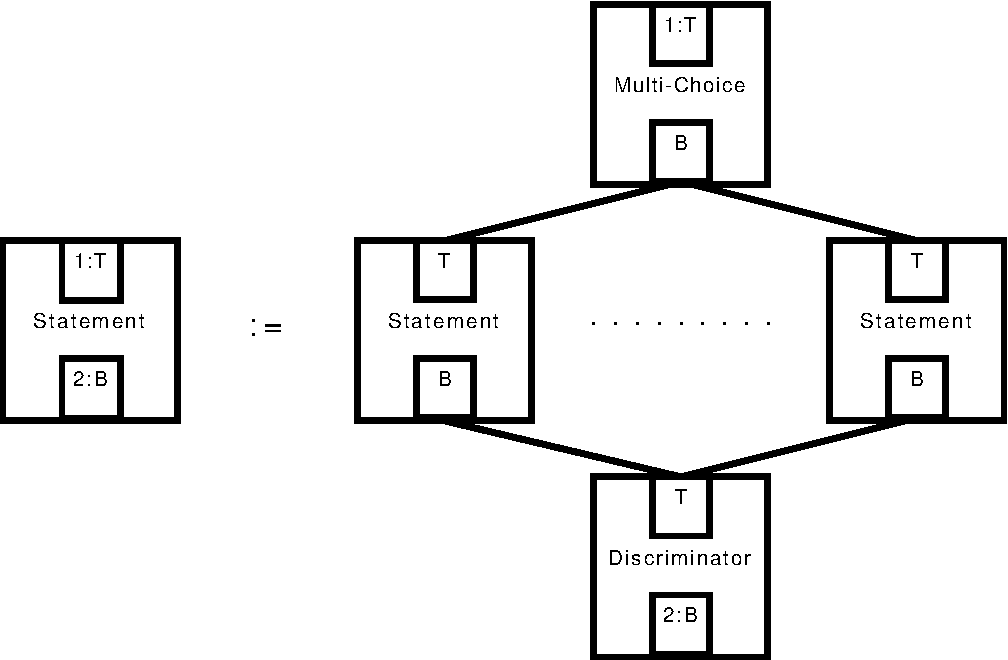
\includegraphics[width=7cm]{figures/grammar/discriminator}\\[5mm]
      \caption[The \emph{Discriminator} grammar rule]{Discriminator}
      \label{figure-grammar-Discriminator}
    \end{center}
  \end{minipage}
\end{figure}

\subsection{Conditions}

The conditions that can be used with branching and input nodes are expressions
built using the following constructs: \emph{Not}, \emph{And}, \emph{Or},
\emph{Xor}, \emph{IsAnything}, \emph{IsArray}, \emph{IsBool}, \emph{IsTrue},
\emph{IsFalse}, \emph{IsFloat}, \emph{IsInteger}, \emph{IsEqual},
\emph{IsNotEqual}, \emph{IsGreaterThan}, \emph{IsEqualOrGreaterThan},
\emph{IsLessThan}, \emph{IsEqualOrLessThan}, \emph{IsObject}, and
\emph{IsString}.

The examples in Appendix~\ref{section-ConditionClasses} show the syntax using
which these constructs can be combined to form condition expressions.

\section{Summary}

This chapter used the workflow patterns to describe the semantics and a graph
grammar to define the syntax of the workflow model that is the foundation for
the software that has been developed as part of this thesis.

The workflow model can be extended, for instance, with support for more
workflow patterns, by adding the respective node types.

\chapter{Design and Implementation}
\label{chapter-DesignAndImplementation}

This chapter discusses the design and implementation of the software that has
been developed as part of this thesis.

\section{Architecture}
\label{section-Architecture}

The workflow engine that has been developed as part of this thesis has been
designed and implemented as three loosely coupled components. The
\texttt{Workflow} component provides an object-oriented framework to define
workflows and an execution engine to execute them.
The \texttt{WorkflowDatabaseTiein} and \texttt{WorkflowEventLogTiein}
components tie the \texttt{Database} and \texttt{EventLog} components from the
eZ~Components library into the main \texttt{Workflow} component for persistence
and monitoring, respectively.

A workflow can be defined programmatically by creating and connecting objects
(see Section~\ref{section-Example}) that represent control flow constructs.
The classes for these objects are provided by the \emph{Workflow Definition API}
(see Appendix~\ref{chapter-API} for a reference). This API also provides the
functionality to save workflow definitions (ie. object graphs) to and load
workflow definitions from a data storage. Two data storage backends have been
implemented, one for relational database systems and another for XML files.
Through the \emph{Workflow Execution API} the execution of a workflow
definition can be started (and resumed). Figure \ref{figure-architecture}
shows the conceptual architecture for the workflow engine.

\clearpage

\begin{figure}[hbt]
\begin{center}
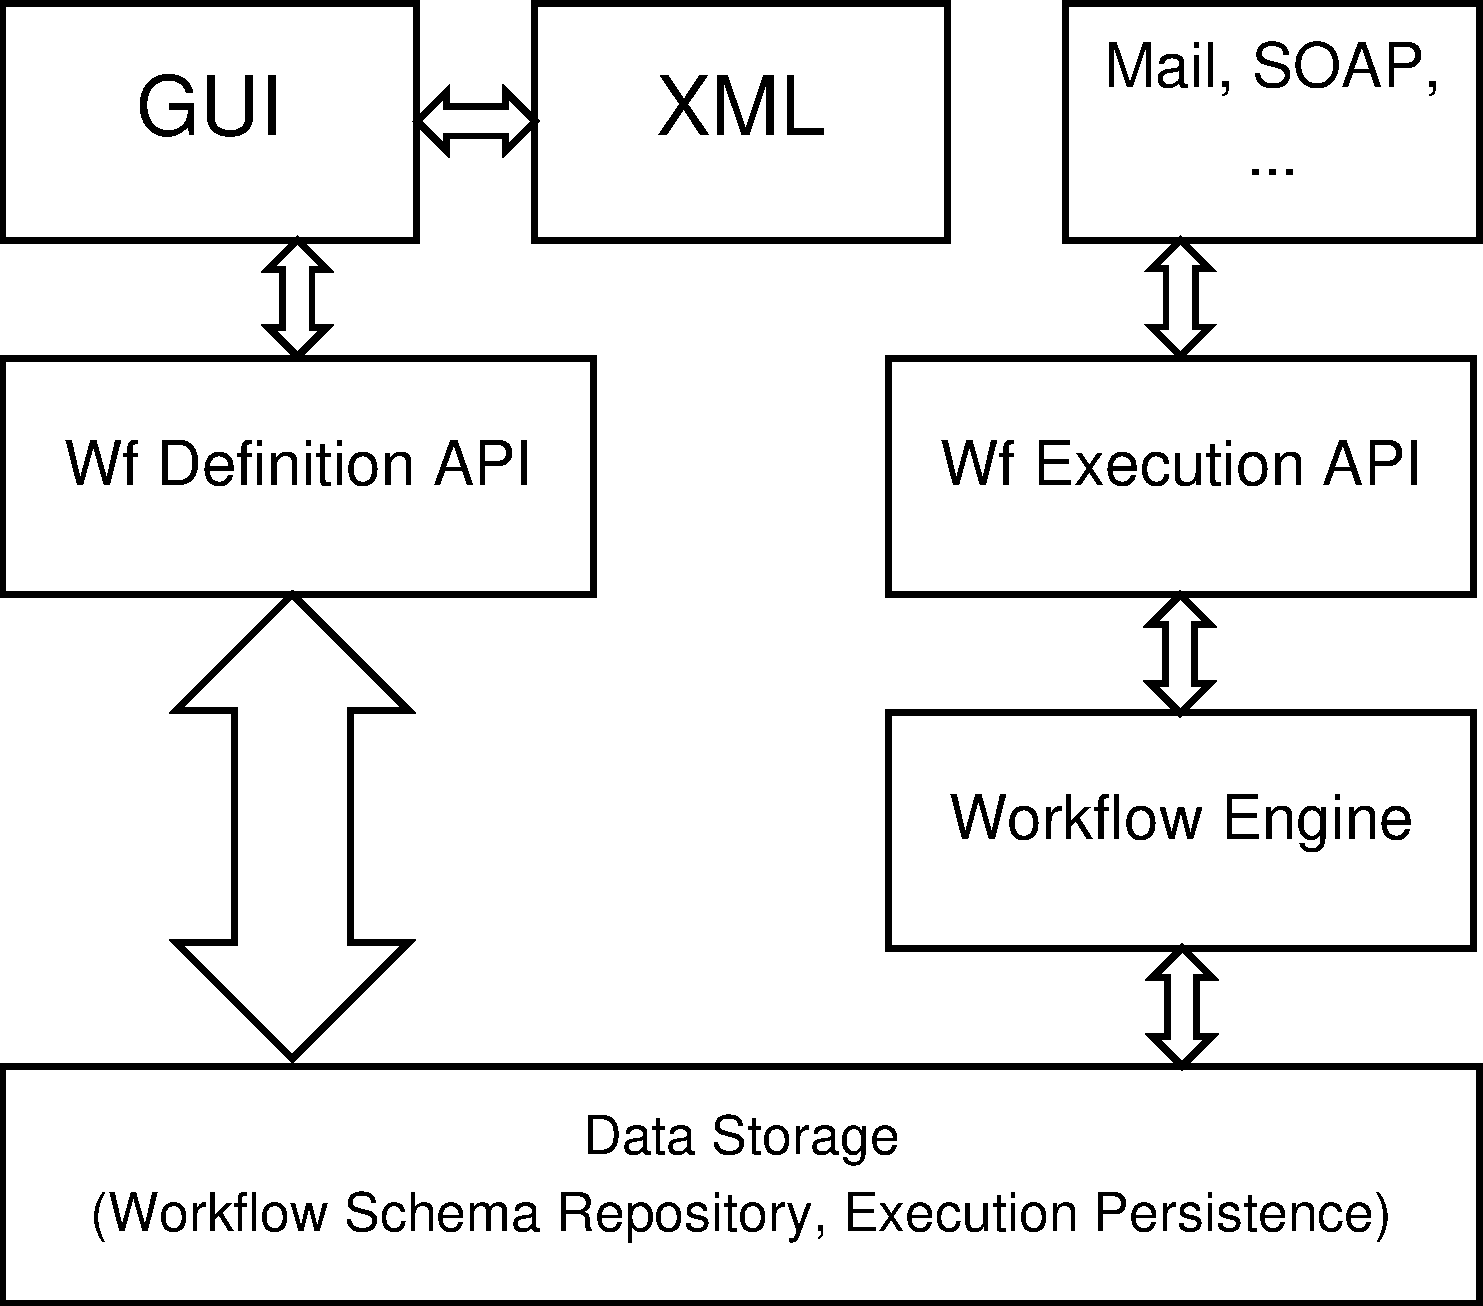
\includegraphics[width=10cm]{figures/architecture}\\[5mm]
\end{center}
\caption{Conceptual architecture for the workflow engine}
\label{figure-architecture}
\end{figure}

The idea that a workflow system should be comprised of loosely coupled
components is discussed, for instance, in \cite{DAM01,DG95,PM99}. Manolescu
states that

\begin{quote}
\emph{an object-oriented workflow architecture must \emph{provide abstractions}
that enable software developers to define and enact how the work flows through
the system} \cite{DAM01}.
\end{quote}

The component-based workflow architecture Micro-Workflow \emph{encapsulates
workflow features in separate components}. This architecture follows the
\emph{Microkernel} pattern which

\begin{quote}
\emph{applies to software systems that must be able to adapt to changing
system requirements. It separates a minimal functional core from extended
functionality and customer-specific parts. The microkernel also serves as a
socket for plugging in these extensions and coordinating their
collaboration} \cite{FB96}.
\end{quote}

The minimalistic core of Micro-Workflow is comprised of three components that
provide basic workflow functionality:

\begin{itemize}
\item The \emph{process component} implements an activity-based workflow model
      and provides the abstractions required to build workflows.
\item The \emph{execution component} implements the functionality to execute
      workflows.
\item The \emph{synchronization component} allows developers to define
      dependencies within the workflow domain.
\end{itemize}

On top of these core components other components, for instance for persistence
(suspending and resuming workflow execution), monitoring (status of running
workflows), history (history of executed workflows), and worklist management
(human-computer interface), can be implemented. Each of these components
\emph{encapsulates a design decision} and can be customized or replaced.

\section{Workflow Virtual Machine}
\label{section-WorkflowVirtualMachine}

This section proposes a so-called \emph{workflow virtual machine} as the
executing component of a component-based workflow architecture.

Given the fact that \emph{standardization efforts, e.g. XPDL \cite{WfMC05}
proposed by the WfMC, have essentially failed to gain universal acceptance}
\cite{WA04}, the \emph{problem of developing a [workflow system] that supports
changes in the [workflow description language]} needs to be addressed.

Fernandes et. al. propose to

\begin{quote}
\emph{split the [workflow system] into two layers: (1) a layer implementing
a \emph{Workflow Virtual Machine}, which is responsible for most of the
[workflow system] activities; and (2) a layer where the different [workflow
description languages] are handled, which is responsible for making the
mapping between each [workflow description language] and the Workflow Virtual
Machine} \cite{SF04}.
\end{quote}

A workflow virtual machine isolates the executing part of a workflow
management system, the \emph{backend}, from the parts that users interact
with, the \emph{frontend}. This isolation allows for the definition of a
\emph{backend language} to describe exactly the workflows that are supported
by the executer and its underlying workflow model. This backend language is
not the workflow description language users use to define their workflows.
They use \emph{frontend languages} that can be mapped to the system's
backend language.

\section{Graph-Oriented Programming}
\label{section-GraphOrientedProgramming}

The manual of JBoss jBPM \cite{JBOSS}, a platform for multiple process
languages supporting workflow, business process management, and process
orchestration, introduces \emph{Graph-Oriented Programming [as a] new
implementation technique that serves as a basis for all graph-based process
languages}.

Graph-Oriented Programming implements the \emph{graphical representation} and
the \emph{wait states} of a process language in an object-oriented programming
language. The former can be achieved by providing a framework of node classes.
Objects of these classes represent the nodes in the process graph, relations
between these objects represent the edges. Such an object graph can then be
traversed for execution. These executions need to be persistable, for instance
in a relational database, to support the wait states.

The aforementioned node classes implement the \emph{Command} design pattern
\cite{GoF94} and encapsulate an action and its parameters.

The executing part of the workflow engine is implemented in an
\texttt{Execution} class. An object of this class represents a workflow in
execution. The execution object has a reference to the current node. When the
execution of a workflow is started, a new execution object is created and the
current node is set to the workflow's start node. The \texttt{execute()}
method that is to be provided by the node classes is not only responsible for
executing the node's action, but also for propagating the execution:
\emph{a node can pass the execution that arrived in the node [to] one of its
leaving transitions to the next node}.

Like Fowler in \cite{MF05}, the authors of the JBoss jBPM manual acknowledge
the fact that \emph{current software development relies more and more on domain
specific languages}. They see Graph-Oriented Programming as a means to
implement domain specific languages \emph{that describe how graphs can be
defined and executed} on top of an object-oriented programming language.

In this context, a process language (like a workflow description language) is
\emph{nothing more than a set of \texttt{Node} implementations}. The semantics
of each node are defined by the implementation of the \texttt{execute()}
method in the respective node class. This language can be used as the backend
language of a Workflow Virtual Machine (see
Section~\ref{section-WorkflowVirtualMachine}). In this lanugage, the workflow
is represented as a graph of command objects. The workflow patterns (see
Section~\ref{section-WorkflowPatterns}) make up the requirements for and can
be mapped to the respective classes.

One of the advantages of using a domain specific language that Fowler gives in
\cite{MF05} regards the \emph{involvement of lay programmers: domain experts
who are not professional programmers but program in domain specific languages
as part of the development effort}. In essence this means that a software
system that provides a domain specific language can be customized and
extended without knowledge of the underlying programming language that was
used to implement it.

\section{Implementation Details}

The workflow engine maintains a set of activated nodes. At the beginning of
the execution, the workflow's start node is activated.

Listing~\ref{listing-ezcWorkflowExecution} shows the main execution loop of
the workflow virtual machine. As long as the workflow execution has not
explicitly ended (by reaching an \emph{End} node), the next activated node
is executed. After the node has been successfully executed it is removed from
the set of activated nodes. In a situation where the set of activated nodes
is not empty but none of the activated nodes can be completed (because they are
waiting for user input, for instance), the workflow execution is suspended.
When the set of activated nodes is empty, the execution of the workflow ends.

\begin{lstlisting}[language=PHP,float,caption={The workflow engine's main execution loop},label=listing-ezcWorkflowExecution]
<?php
abstract class ezcWorkflowExecution
{
    // ...

    protected function execute()
    {
        do
        {
            $executed = false;

            foreach ( $this->activatedNodes as $key => $node )
            {
                if ( !$this->hasEnded() )
                {
                    if ( $node->execute( $this ) )
                    {
                        unset( $this->activatedNodes[$key] );
                        $executed = true;
                    }
                }
            }
        }
        while ( !empty( $this->activatedNodes ) && $executed );

        if ( !$this->hasEnded() )
        {
            $this->suspend();
        }
    }

    // ...
}
?>
\end{lstlisting}

During its execution, a node can activate an arbitrary amount of its outgoing
nodes. \emph{Synchronization}, \emph{Synchronizing Merge}, and
\emph{Discriminator} nodes, for instance, need to be activated several times
before they can complete their execution.

Parallel threads of execution that are branched by the \emph{Parallel Split}
and \emph{Multi-Choice} (and merged by the \emph{Synchronization},
\emph{Synchronizing Merge}, and \emph{Discriminator}) workflow patterns are
executed serialized.

\clearpage
\section{Example}
\label{section-Example}

Listing~\ref{listing-Example.php} shows an example of PHP code that
programmatically creates an object graph for a workflow.

\begin{lstlisting}[language=PHP,float,caption={Creating an object graph using the \emph{Workflow Definition API}},label=listing-Example.php]
<?php
require_once 'Base/base.php';

function __autoload( $className )
{
    ezcBase::autoload( $className );
}

$workflow = new ezcWorkflow( 'Test' );

$input = new ezcWorkflowNodeInput(
  array(
    'choice' => 'boolean'
  )
);

$workflow->startNode->addOutNode( $input );

$branch = new ezcWorkflowNodeExclusiveChoice;
$branch->addInNode( $input );

$true  = new ezcWorkflowNodeAction( 'PrintTrue' );
$false = new ezcWorkflowNodeAction( 'PrintFalse' );

$branch->addConditionalOutNode(
  new ezcWorkflowConditionIsTrue(
    'choice'
  ),
  $true
);

$branch->addConditionalOutNode(
  new ezcWorkflowConditionIsFalse(
    'choice'
  ),
  $false
);

$merge = new ezcWorkflowNodeSimpleMerge;
$merge->addInNode( $true )
      ->addInNode( $false )
      ->addOutNode( $workflow->endNode );
?>
\end{lstlisting}

The workflow in this example consists of seven nodes:

\begin{enumerate}
\item A \emph{Start} node (line 10).
\item An \emph{Input} node (lines 13--17) that requests a boolean input
      variable.
\item An \emph{Exclusive Choice} node (line 21) that conditionally
      branches (lines 27--39) based upon the value of the previously
      supplied input variable.
\item An \emph{Action} node that has a \texttt{PrintTrue} service
      object attached to it (line 24).
\item An \emph{Action} node that has a \texttt{PrintFalse} service
      object attached to it (line 25).
\item A \emph{Simple Merge} node (lines 41--44).
\item An \emph{End} node (line 11).
\end{enumerate}

Listing~\ref{listing-XML} shows the object graph created by this PHP code
serialized to XML, Appendix~\ref{chapter-Tutorial} elaborates on this example
and explains it in detail.

\begin{lstlisting}[language=XML,firstnumber=1,stepnumber=100,float,caption={Workflow specification in XML markup},label=listing-XML]
<?xml version="1.0" encoding="UTF-8"?>

<workflow name="Test" version="1">
  <node id="1" type="Start">
    <outNode id="3"/>
  </node>

  <node id="2" type="End"/>

  <node id="3" type="Input">
    <variable name="choice" constraint="boolean"/>
    <outNode id="4"/>
  </node>

  <node id="4" type="ExclusiveChoice">
    <condition type="IsTrue" variable="choice">
      <outNode id="5"/>
    </condition>

    <condition type="IsFalse" variable="choice">
      <outNode id="6"/>
    </condition>
  </node>

  <node id="5" type="Action" serviceObjectClass="PrintTrue">
    <outNode id="7"/>
  </node>

  <node id="6" type="Action" serviceObjectClass="PrintFalse">
    <outNode id="7"/>
  </node>

  <node id="7" type="SimpleMerge">
    <outNode id="2"/>
  </node>
</workflow>
\end{lstlisting}

\clearpage
\section{Summary}

The core of the workflow engine that has been developed as part of this thesis
is a virtual machine that executes workflows represented through object graphs.
These object graphs can be created programmatically through the software
component's Workflow Definition API. Alternatively, a workflow definition can
be loaded from an XML file. Object graph and XML file are two different
representations of a workflow definition that uses the so-called backend
language of the workflow engine's core. Arbitrary frontend languages such as
the XML Process Definition Language (XPDL) \cite{WfMC05}, for instance, can be
mapped to the workflow engine's backend language.

\chapter{Evaluation and Related Work}
\label{chapter-Evaluation}

This chapter evaluates the workflow model (see
Chapter~\ref{chapter-WorkflowModel}) and the software (see
Chapter~\ref{chapter-DesignAndImplementation}) that have been developed as
part of this with regard to the requirements (see
Chapter~\ref{chapter-Requirements}) and compares it related work.

\section{Evaluation}

\subsection{Workflow Model}

The workflow model (see Chapter~\ref{chapter-WorkflowModel}) that is the basis
of the software that has been developed as part of this thesis meets the
requirements set up by eZ~Systems~AS (see
Section~\ref{section-RequirementseZPublishTelemark}). It provides good support
for expressing control flow with its direct support of the basic control flow
patterns (see Section~\ref{subsection-BasicControlFlowPatterns}) and the
workflow patterns for advanced branching and synchronization (see
Section~\ref{subsection-AdvancedBranchingAndSynchronization}). This allows the
expression of operations such as the publishing, removal, and modification of
content objects in eZ~Publish to be expressed through workflows. The support
of sub-workflows allows the decomposition of these workflows into manageable
and reusable parts.

Table~\ref{table-ComparisonWorkflowSystems} compares the expressiveness of
the \texttt{ezcWorkflow} components's \emph{backend language} with regard to
the directly supported workflow patterns to other workflow systems. The
comparison data is partially taken from \cite{BK03}.

\begin{table}[hbtp]
\begin{center}
\begin{tabular}[t]{|p{100pt}|l|l|l|l|l|l|l|l|l|l|l|l|l|}
\hline
\small{\textbf{Workflow Pattern}} &
\begin{sideways}\small{\textbf{ezcWorkflow}}\end{sideways} &
\begin{sideways}\small{\textbf{YAWL}}\end{sideways} &
\begin{sideways}\small{\textbf{eZ Publish 3}}\end{sideways} &
\begin{sideways}\small{\textbf{Galaxia}}\end{sideways} &
\begin{sideways}\small{\textbf{Radicore}}\end{sideways} &
\begin{sideways}\small{\textbf{Visual WorkFlo}}\end{sideways} &
\begin{sideways}\small{\textbf{Verve Workflow}}\end{sideways} &
\begin{sideways}\small{\textbf{Staffware}}\end{sideways} &
\begin{sideways}\small{\textbf{MQSeries Workflow}}\end{sideways} &
\begin{sideways}\small{\textbf{Fort� Conductor}}\end{sideways} &
\begin{sideways}\small{\textbf{HP ChangeEngine}}\end{sideways} &
\begin{sideways}\small{\textbf{Fujitsu i-Flow}}\end{sideways} &
\begin{sideways}\small{\textbf{SAP R/3 Workflow}}\end{sideways} \\
\hline
\small{Sequence} & \small{$\surd$} & \small{$\surd$} & \small{$\surd$} & \small{$\surd$} & \small{$\surd$} & \small{$\surd$} & \small{$\surd$} & \small{$\surd$} & \small{$\surd$} & \small{$\surd$} & \small{$\surd$} & \small{$\surd$} & \small{$\surd$} \\
\hline
\small{Parallel Split} & \small{$\surd$} & \small{$\surd$} & (\small{$\surd$}) & \small{$\surd$} & \small{$\surd$} & \small{$\surd$} & \small{$\surd$} & \small{$\surd$} & \small{$\surd$} & \small{$\surd$} & \small{$\surd$} & \small{$\surd$} & \small{$\surd$} \\
\hline
\small{Synchronization} & \small{$\surd$} & \small{$\surd$} & & \small{$\surd$} & \small{$\surd$} & \small{$\surd$} & \small{$\surd$} & \small{$\surd$} & \small{$\surd$} & \small{$\surd$} & \small{$\surd$} & \small{$\surd$} & \small{$\surd$} \\
\hline
\small{Exclusive Choice} & \small{$\surd$} & \small{$\surd$} & & \small{$\surd$} & \small{$\surd$} & \small{$\surd$} & (\small{$\surd$}) & \small{$\surd$} & (\small{$\surd$}) & \small{$\surd$} & \small{$\surd$} & \small{$\surd$} & \small{$\surd$} \\
\hline
\small{Simple Merge} & \small{$\surd$} & \small{$\surd$} & & (\small{$\surd$}) & \small{$\surd$} & \small{$\surd$} & \small{$\surd$} & \small{$\surd$} & \small{$\surd$} & \small{$\surd$} & \small{$\surd$} & \small{$\surd$} & \small{$\surd$} \\
\hline
\small{Multi-Choice} & \small{$\surd$} & \small{$\surd$} & & & & (\small{$\surd$}) & \small{$\surd$} & (\small{$\surd$}) & \small{$\surd$} & \small{$\surd$} & \small{$\surd$} & (\small{$\surd$}) & (\small{$\surd$}) \\
\hline
\small{Synchronizing Merge} & \small{$\surd$} & \small{$\surd$} & & & \small{$\surd$} & & & \small{$\surd$} & & & & & \\
\hline
\small{Multi-Merge} & & \small{$\surd$} & & & & & \small{$\surd$} & & & \small{$\surd$} & & & \\
\hline
\small{Discriminator} & \small{$\surd$} & \small{$\surd$} & & & & & \small{$\surd$} & & & (\small{$\surd$}) & \small{$\surd$} & & \small{$\surd$} \\
\hline
\small{Arbitrary Cycles} & \small{$\surd$} & \small{$\surd$} & & & \small{$\surd$} & & \small{$\surd$} & \small{$\surd$} & & \small{$\surd$} & \small{$\surd$} & \small{$\surd$} & \\
\hline
\small{Implicit Termination} & \small{$\surd$} & & & & & & & \small{$\surd$} & \small{$\surd$} & & & & \\
\hline
\small{Multiple Instances without Synchronization} & & \small{$\surd$} & & & & \small{$\surd$} & \small{$\surd$} & & & \small{$\surd$} & & \small{$\surd$} & \\
\hline
\small{Multiple Instances with A Priori Design Time Knowledge} & & \small{$\surd$} & & & & \small{$\surd$} & \small{$\surd$} & \small{$\surd$} & \small{$\surd$} & \small{$\surd$} & \small{$\surd$} & \small{$\surd$} & \small{$\surd$} \\
\hline
\small{Multiple Instances with A Priori Runtime Knowledge} & & \small{$\surd$} & & & & & & & & & & & (\small{$\surd$}) \\
\hline
\small{Multiple Instances without A Priori Runtime Knowledge} & & \small{$\surd$} & & & & & & & & & & & \\
\hline
\small{Deferred Choice} & & \small{$\surd$} & & & & & & (\small{$\surd$}) & & & & & \\
\hline
\small{Interleaved Parallel Routing} & & \small{$\surd$} & & & & & & & & & & & \\
\hline
\small{Milestone} & & \small{$\surd$} & & & & & & & & & & & \\
\hline
\small{Cancel Activity} & & \small{$\surd$} & & & & & & \small{$\surd$} & & & & & \small{$\surd$} \\
\hline
\small{Cancel Case} & \small{$\surd$} & \small{$\surd$} & & & & \small{$\surd$} & \small{$\surd$} & & & \small{$\surd$} & \small{$\surd$} & & \small{$\surd$} \\
\hline
\end{tabular}
\caption{Comparison of Workflow Systems}
\label{table-ComparisonWorkflowSystems}
\end{center}
\end{table}

\subsection{Implementation}

The software that has been developed as part of this thesis meets the
requirements set up by eZ~Systems~AS (see
Section~\ref{section-RequirementseZPublishTelemark}). It has been
implemented using version~5 of the PHP programming language and is
customizable and extendable. Its architecture allows the addition and
customization of components for workflow execution, persistence, history,
monitoring, and worklist management, for instance. The backend language
that is understood by its virtual machine can be extended by implementing
new node classes. The data storage for workflow schemas and the persistence
of workflow instances has been abstracted, reference implementations for
relational databases (workflow schemas and persistence) and XML files
(workflow schemas only) are available. The workflow schemas are stored in
such a way that they are versioned, old and new versions of a workflow can
be executed at the same time. The \emph{Workflow Execution API} provides
access to information on the workflow instances that are currently
executing and it is possible to manually control the workflow instances
that are currently executing. Through PHP's native SOAP support, the
\emph{Workflow Execution API} can be exposed as a web service, thus
faciliating a distributed and federated workflow environment where one
workflow on one server can start another workflow on another server, for
instance. A special purpose implementation of the workflow virtual machine,
\texttt{ezcWorkflowTestExecution}, allows for the simulation of workflow
execution for debugging and testing.

\section{Related Work}

\subsection{Research}

\subsubsection{Micro-Workflow}

Manolescu proposes \emph{a new workflow architecture that bridges the gap
between the type of functionality provided by current workflow systems and
the type of workflow functionality required in object-oriented applications}.
In his PhD thesis \cite{DAM01}, he discusses the design and implementation of
Micro-Workflow, an object-oriented framework that is built using this
architecture. One of Manolescu's key findings is that more advanced workflow
features can be added to light-weight workflow core through composition.

\subsubsection{SWAMP}

In his Diploma thesis \cite{TS04}, Schmidt discusses the design and
implementation of the SWAMP workflow system (SuSE Workflow and Management
Platform). The goal of Schmidt's thesis is to replace an inhomogeneous
legacy system with a unified workflow system that is easier to maintain and
that can be easily customized and extended. The motivations behind and the
requirements for the SWAMP workflow system have some similarities with the
needs for the software that has been developed as part of this thesis.

\subsubsection{YAWL}

In her Master thesis \cite{SH05}, Heijens discusses the design and
implementation of YAWL. YAWL is both a workflow language (Yet Another Workflow
Language) and a workflow system. The workflow model of YAWL is formally based
on Petri nets and supports all the workflow patterns with the exception of
\emph{Implicit Termination}.

\subsection{Workflow Systems for PHP}

\subsubsection{eZ Publish 3}

From the workflow patterns that were discussed in
Section~\ref{section-WorkflowPatterns}, the workflow system of eZ~Publish~3
only supports the \emph{Sequence} workflow pattern directly. Through its
\emph{Multiplexer} workflow event, which starts another workflow from within
a workflow, it indirectly supports the \emph{Parallel Split} workflow pattern.

The technical limitations of the workflow system in eZ~Publish~3 (see
Section~\ref{section-RequirementseZPublish3}) are representative for other
content management systems for the PHP platform (and most likely for those for
other platforms as well). The tight integration with the application into
which the workflow system is embedded makes the independent usage of the
workflow system impossible.

\subsubsection{Galaxia Workflow Engine}

The Galaxia Workflow Engine \cite{GF03} is an activity-based workflow engine
for PHP that is loosely based on OpenFlow \cite{OPENFLOW}.

The graphical workflow description language supported by the Galaxia workflow
engine consists of six \emph{activity types}:

\begin{enumerate}
\item \emph{Start} represents the beginning of a workflow.
\item \emph{End} represents the end of a workflow.
\item \emph{Activity} represents an activity that is to be performed.
\item \emph{Switch} represents a point of decision in the workflow and can be
      compared to the \emph{Exclusive Choice} workflow pattern.
\item \emph{Split} is equivalent to the \emph{Parallel Split} workflow
      pattern.
\item \emph{Join} is equivalent to the \emph{Synchronization} workflow
      pattern.
\end{enumerate}

Galaxia does not have an explicit \emph{Simple Merge} construct to merge
the multiple possible threads of a \emph{Switch} construct. Instead, an
\emph{Activity} construct implicitly merges its incoming threads.

\subsubsection{Radicore}

The Radicore toolkit for PHP features an activity-based workflow engine that
is based on Petri nets \cite{TM04}.

It supports

\begin{itemize}
\item Sequential Routing.
\item Parallel Routing through \emph{AND-Split} and \emph{AND-Join} constructs.
\item Conditional Routing through explicit and implicit \emph{OR-Split} and
      \emph{OR-Join} constructs.
\item Iterative Routing using the \emph{OR-Split} construct.
\end{itemize}

These constructs correspond to the \emph{Sequence}, \emph{Parallel Split},
\emph{Synchronization}, \emph{Exclusive Choice}, and \emph{Simple Merge}
workflow patterns (see Section~\ref{section-WorkflowPatterns}).

\section{Summary}

Workflow systems such as Micro-Workflow \cite{DAM01} and YAWL \cite{SH05}, for
instance, that have been implemented as part of academic research often excel
only in the aspect that is specific to the research while neglecting other
aspects that are relevant to a workflow system. One of the goals of this
thesis was to combine aspects such as component-based workflow architecture,
workflow virtual machine, and workflow patterns to create a workflow system
that meets industry requirements.

The existing workflow systems for PHP do not lend themselves well to
customization and extension with regard to the requirements set up by
eZ~Systems~AS. This fact, together with eZ~Systems' requirement for clear
intellectual property, lead to the development of a new workflow engine
instead of starting with an existing one.

\chapter{Conclusion and Future Work}
\label{chapter-Conclusion}

\section{Conclusion}

This thesis reviewed previous research such as \cite{BK03,DAM01,PM99,SF04}
and combined it for the first time in an effort to design and implement a
workflow system that meets industry requirements.

The pragmatic approach to describe the semantics of workflow routing constructs
through \emph{Workflow Patterns} \cite{BK03} provides a good foundation for the
\emph{Backend Language} of a \emph{Workflow Virtual Machine} \cite{SF04} that
executes workflow definitions represented through object graphs in a
component-based workflow architecture \cite{DAM01}.

The software that has been developed as part of this thesis is a contribution
to the PHP community. It provides an extendable framework to define workflows
and a virtual machine for the execution of these definitions that can be
embedded into a PHP application, thus extending it with workflow capabilities.
This workflow system can be customized and extended through the composition of
components, its workflow model can be customized and extended through the
classes that define the control flow constructs. It is neither bound to a
specific application into which it is embedded nor to a specific workflow
description language, thus providing more degrees of freedom with regard to
use -- and re-use -- of the workflow engine.

\section{Future Work}

\subsection{Analysis and Verification of Workflows}

The current implementation of the software that has been developed as part of
this thesis has basic support for the analysis and verification of workflow
specifications. Future versions of the software can implement more advanced
verification tools based upon the \emph{abundance of analysis techniques} that
exists for Petri nets \cite{WA96}.

\subsection{Workflow Model}

The workflow model can be extended, for instance, with support for more
workflow patterns, by adding the respective node types.

\subsection{Aspect-Oriented Programming}

Aspect-Oriented Programming \emph{allow[s] programming by making quantified
programmatic assertions over programs written by programmers oblivious to
such assertions} \cite{RF00}. These assertions make \emph{quantified
statements about which code is to execute in which circumstances}.

Section 2 of \cite{SB06} presents an overview of the various implementations
of AOP for PHP that support AOP by extending the base programming language.
The combination of Graph-Oriented Programming with Aspect-Oriented Programming
would add yet another possibility to faciliate AOP with the PHP platform, but
without the need to change or extend the base programming language. The
workflow model discussed in Chapter~\ref{chapter-WorkflowModel} would serve as
the Joinpoint Model of an AOP system that can be implemented as an additional
component for the software that was presented in
Chapter~\ref{chapter-DesignAndImplementation}. Pointcuts such as \emph{node of
type X is executed} could then be used to express when additional code is to
be run during workflow execution. Compared to the implicit callgraph structure
on which language-level AOP systems operate, the explicit graph structure of
workflows makes the idea of AOP intuitively clear.

This combination of Aspect-Oriented Programming with Graph-Oriented Programming
could then be compared to Aspect-Oriented Programming in general as well as
to Adaptive Programming which Lieberherr describes as \emph{thespecial case of
Aspect-Oriented Programming (AOP) where some of the building blocks are
expressible in terms of graphs} \cite{KL97}.

\subsection{Compilation of Workflows}

Model-Driven Architecture (MDA) \emph{separates business and application logic
from underlying platform technology} \cite{JM01} and supports the Model-Driven
Engineering (MDE) of software systems. It offers a \emph{promising approach to
address the inability of third-generation languages to alleviate the complexity
of platforms and express domain concepts effectively} \cite{DS06}.

In this context the possibility could be evaluated whether the software that
has been developed as part of this thesis can be extended with a code
generator component that can compile a workflow specification into a
ready-to-use application.


\begin{appendix}

\chapter{Tutorial}
\label{chapter-Tutorial}

This appendix serves as an introduction to the \emph{Workflow Definition API}
and \emph{Workflow Execution API} (see Figure \ref{figure-architecture}).

\section{Workflow Definition API}

\subsection{Defining a New Workflow}

In this subsection, we define a new workflow by creating an object graph of
\texttt{ezcWorkflowNode} objects. Once we learned how to define and store such
a workflow definition, we we will look at loading and editing an existing
workflow definition.

\subsubsection{Creating the Object Graph}

First, we load the \texttt{ezcBase} component (line 2) and set up its
classloader that is based on PHP's \texttt{\_\_autoload} interceptor
(lines 4--7).

\begin{lstlisting}[language=PHP,firstnumber=1]
<?php
require_once 'Base/base.php';

function __autoload( $className )
{
    ezcBase::autoload( $className );
}
\end{lstlisting}

For the following code listings, lines 1--7 will always be the same as in the
listing above.

We create a new object of the \texttt{ezcWorkflow} class (line 8). This object
represents the workflow that we are about to define. The constructor of the
class expects a string with a name for the workflow. This name is unique for
the schema repository to which the workflow may be saved later.

\begin{lstlisting}[language=PHP,firstnumber=8]
$workflow = new ezcWorkflow( 'Test' );
\end{lstlisting}

We define an \emph{Input} node by creating an object of the
\texttt{ezcWorkflowNodeInput} class. The constructor expects an associative
array where the key stands for the name of an input variable and the value
may hold arbitrary expectations for this variable. These expectations are
evaluated and checked by the application that uses the workflow component.

Then we set up the \emph{Input} node as an outgoing node of the \emph{Start}
node.

\begin{lstlisting}[language=PHP,firstnumber=9]
$input = new ezcWorkflowNodeInput(
  array(
    'choice' => new ezcWorkflowConditionIsBool
  )
);

$workflow->startNode->addOutNode( $input );
\end{lstlisting}

For the purposes of this example we assume that \texttt{'choice' => 'boolean'}
means that a boolean input variable of name ''choice'' is expected.

We now define an \emph{Exclusive Choice} node that uses the value of the input
variable to activate one of two possible paths. Before we set up its outgoing
nodes (and the related conditions), we set up the \emph{Exclusive Choice} as
an outgoing node of the \emph{Input} node (lines 16--17).

\begin{lstlisting}[language=PHP,firstnumber=16]
$branch = new ezcWorkflowNodeExclusiveChoice;
$branch->addInNode( $input );
\end{lstlisting}

In the next step, we create two objects, \texttt{\$true} and \texttt{\$false}
of the \texttt{ezcWorkflowNodeAction} class (lines 18--19). The constructor
expects the name of a class that implements the\\ \texttt{ezcWorkflowServiceObject}
interface. Such a class encapsulates the business logic that is associated with the
\emph{Action} node.

\begin{lstlisting}[language=PHP,firstnumber=18]
$true  = new ezcWorkflowNodeAction( 'PrintTrue' );
$false = new ezcWorkflowNodeAction( 'PrintFalse' );
\end{lstlisting}

Let us take a look at what an implementation of the
\texttt{ezcWorkflowServiceObject} interface looks like:

\begin{quote}
\begin{lstlisting}[language=PHP,firstnumber=1,stepnumber=100]
<?php
class PrintTrue implements ezcWorkflowServiceObject
{
    public function execute( ezcWorkflowExecution $e )
    {
        print "TRUE\n";
    }

    public function __toString()
    {
        return 'PrintTrue';
    }
}
?>
\end{lstlisting}

The \texttt{ezcWorkflowServiceObject} interface requires two methods,
\texttt{execute()} and \texttt{\_\_toString()}. The former implements the
business logic of the service object and is passed the execution context as
its only argument. The latter provides a textual representation of the
service object.
\end{quote}

Using the \texttt{\$branch} object's \texttt{addConditionalOutNode()} method,
we can now set up the \emph{Action} node that is represented by the
\texttt{\$true} object as an conditional outgoing node (lines 20--26). This
method expects an \texttt{ezcWorkflowCondition} object as its first argument.
This object encapsulates the branching condition.

For our example we use the \texttt{ezcWorkflowConditionIsTrue} class. The
constructor of this class expects the name of a workflow variable that is to
be evaluated.

\begin{lstlisting}[language=PHP,firstnumber=20]
$branch->addConditionalOutNode(
  new ezcWorkflowConditionVariable(
    'choice',
    new ezcWorkflowConditionIsTrue
  ),
  $true
);
\end{lstlisting}

Section~\ref{section-ConditionClasses} shows the available
\texttt{ezcWorkflowCondition} implementations.

Analogous, we set up the \emph{Action} node that is represented by the
\texttt{\$false} object as a second conditional outgoing node (lines 27--33).

\begin{lstlisting}[language=PHP,firstnumber=27]
$branch->addConditionalOutNode(
  new ezcWorkflowConditionVariable(
    'choice',
    new ezcWorkflowConditionIsFalse
  ),
  $false
);
\end{lstlisting}

Finally, we create a new object of the \texttt{ezcWorkflowNodeSimpleMerge}
class (line 34). We set up the two \emph{Action} nodes as incoming nodes and the
\emph{End} node as an outgoing node of this \emph{Simple Merge} node (lines 35--37).

\begin{lstlisting}[language=PHP,firstnumber=34]
$merge = new ezcWorkflowNodeSimpleMerge;
$merge->addInNode( $true )
      ->addInNode( $false )
      ->addOutNode( $workflow->endNode );
\end{lstlisting}

This concludes the creation of the object graph that represents the workflow
specification and can now be stored in a workflow schema repository. Currently
two workflow schema repository backends are supported, XML files and relational
databases.

\subsubsection{Writing the Workflow Schema to an XML File}

The following code snippet demonstrates how to serialize the object graph to
an XML representation.

\begin{lstlisting}[language=PHP,firstnumber=38]
$definition = new ezcWorkflowDefinitionStorageXml;
$definition->save( $workflow );
?>
\end{lstlisting}

The constructor of the \texttt{ezcWorkflowDefinitionStorageXml} class accepts an
optional argument that specifies the directory in which the XML files are
stored.

Listing \ref{listing-XML2} shows the resulting XML document that is written to
a file named \texttt{Test\_1.xml}. The filename includes the name of the
workflow definition and its version number.

\begin{lstlisting}[language=XML,firstnumber=1,stepnumber=100,float,caption={Workflow specification in XML markup},label=listing-XML2]
<?xml version="1.0" encoding="UTF-8"?>

<workflow name="Test" version="1">
  <node id="1" type="Start">
    <outNode id="3"/>
  </node>

  <node id="2" type="End"/>

  <node id="3" type="Input">
    <variable name="choice">
      <condition type="IsBool"/>
    </variable>
    <outNode id="4"/>
  </node>

  <node id="4" type="ExclusiveChoice">
    <condition type="Variable" name="choice">
      <condition type="IsTrue"/>
      <outNode id="5"/>
    </condition>

    <condition type="Variable" name="choice">
      <condition type="IsFalse"/>
      <outNode id="6"/>
    </condition>
  </node>

  <node id="5" type="Action" serviceObjectClass="PrintTrue">
    <outNode id="7"/>
  </node>

  <node id="6" type="Action" serviceObjectClass="PrintFalse">
    <outNode id="7"/>
  </node>

  <node id="7" type="SimpleMerge">
    <outNode id="2"/>
  </node>
</workflow>
\end{lstlisting}

Frontend languages such as the XML Process Definition Language (XPDL)
\cite{WfMC05} can be transformed to this format using XSL Transformations
(XSLT) \cite{W3C07}, for instance.

\subsubsection{Saving the Workflow Schema to a Database}

The constructor of the \texttt{ezcWorkflowDatabaseDefinition} class expects
and object of the \texttt{ezcDbHandler} class. In line 38 we create such an
object and connect to a MySQL database server. Then we can use the
\texttt{save()} method of the \texttt{ezcWorkflowDatabaseDefinition} object
to save the object graph to the database.

\begin{lstlisting}[language=PHP,firstnumber=38]
$db         = ezcDbFactory::create( 'mysql://test@localhost/test' );
$definition = new ezcWorkflowDatabaseDefinition( $db );
$definition->save( $workflow );
?>
\end{lstlisting}

\subsubsection{Visualizing a Workflow Graph}

The next code snippet shows how to use the \texttt{ezcWorkflowVisitorVisualization}
class to generate a description of the object graph in the DOT graph description
language.

\begin{lstlisting}[language=PHP,firstnumber=38]
$visitor = new ezcWorkflowVisitorVisualization;
$workflow->accept( $visitor );
print $visitor;
?>
\end{lstlisting}

Listing~\ref{listing-DOT} shows the resulting DOT graph description,
Figure~\ref{figure-GraphVizExample} shows the workflow graph rendered using
GraphViz from this graph description.

\begin{lstlisting}[firstnumber=1,stepnumber=100,float,caption={Workflow specification in DOT markup},label=listing-DOT]
digraph Test {
node1 [label="Start"]
node3 [label="Input"]
node4 [label="Exclusive Choice"]
node5 [label="PrintTrue"]
node7 [label="Simple Merge"]
node2 [label="End"]
node6 [label="PrintFalse"]

node1 -> node3
node3 -> node4
node4 -> node5 [label="choice is true"]
node4 -> node6 [label="choice is false"]
node5 -> node7
node7 -> node2
node6 -> node7
}
\end{lstlisting}

\begin{figure}[hbt]
\begin{center}
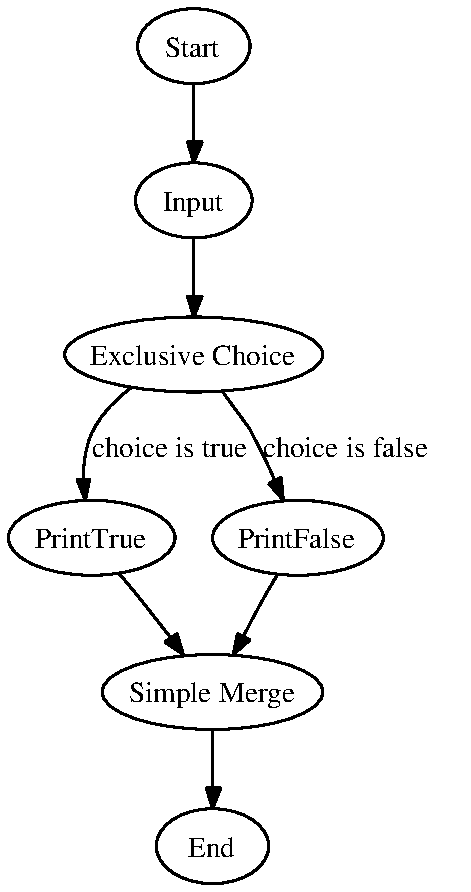
\includegraphics[width=7cm]{figures/GraphVizExample}\\[5mm]
\end{center}
\caption{Workflow graph rendered using GraphViz}
\label{figure-GraphVizExample}
\end{figure}

\subsection{Loading an Existing Workflow}

\subsubsection{Loading a Workflow Schema from an XML File}

The following code snippet demonstrates how to load an object graph from
an XML representation.

\begin{lstlisting}[language=PHP,firstnumber=8]
$definition = new ezcWorkflowDefinitionStorageXml;
$workflow   = $definition->loadByName( 'Test' );
?>
\end{lstlisting}

The \texttt{loadByName()} method accepts an optional second argument that
specifies the version number of the workflow definition that is to be loaded.
By default (ie. without the second argument) the newest version of the workflow
is loaded.

\subsubsection{Loading a Workflow Schema from a Database}

Loading a workflow schema from a database is analogous to loading fron an XML
file:

\begin{lstlisting}[language=PHP,firstnumber=8]
$db         = ezcDbFactory::create( 'mysql://test@localhost/test' );
$definition = new ezcWorkflowDatabaseDefinition( $db );
$workflow   = $definition->loadByName( 'Test' );
\end{lstlisting}

For the following code listings, lines 8--10 will always be the same as in the
listing above.

\section{Workflow Execution API}

The software that has been developed as part of this thesis offers three
workflow execution engines: \texttt{ezcWorkflowExecutionNonInteractive},
\texttt{ezcWorkflowDatabaseExecution}, and \texttt{ezcWorkflowTestExecution}.
This sections shows how they are used.

\subsection{Workflow with Wait States}

For the execution of a workflow that contains wait states (for example
\emph{Input} nodes), an execution engine is required that supports
persistence. The \texttt{ezcWorkflowDatabaseExecution} class implements
such an execution engine and uses a relational database for persistence
storage.

In the following code snippet we start start the execution of a previously
loaded workflow.

\begin{lstlisting}[language=PHP,firstnumber=11]
$execution = new ezcWorkflowDatabaseExecution( $db );
$execution->workflow = $workflow;
$executionId = $execution->start();
\end{lstlisting}

As our workflow contains an \emph{Input} node, the execution will not complete
and will be suspended. The \texttt{\$executionId} uniquely identifies the
suspended workflow execution. It can be used, for instance, to resume the
workflow execution once the requested input data has been provided:

\begin{lstlisting}[language=PHP,firstnumber=14]
$execution = new ezcWorkflowDatabaseExecution( $db );
$execution->resume( $executionId, array( 'choice' => true ) );
?>
\end{lstlisting}

\subsection{Workflow without Wait States}

A workflow that contains no wait states can be executed in one pass. The
workflow engine is not required to support persistence for this. The
\texttt{ezcWorkflowExecutionNonInteractive} class implements a workflow
engine without persistence support that can execute such workflow without
the overhead of a persistence layer.

\begin{lstlisting}[language=PHP,firstnumber=11]
$execution = new ezcWorkflowExecutionNonInteractive;
$execution->workflow = $workflow;
$execution->start();
?>
\end{lstlisting}

\subsection{Simulating Workflow Execution}

The workflow engine implemented by the \texttt{ezcWorkflowTestExecution}
class can be used for testing both the workflow system itself as well as
workflow definitions.

\begin{lstlisting}[language=PHP,firstnumber=11]
$execution = new ezcWorkflowTestExecution;
$execution->workflow = $workflow;
$execution->setInputVariable( 'choice', true );
$execution->start();
?>
\end{lstlisting}

The \texttt{setInputVariable()} method allows for the mocking of
\emph{Input} nodes, thus making it possible to execute and test interactive
workflows without interaction.

\chapter{API Reference}
\label{chapter-API}

This appendix provides an API reference for the software that has been
developed as part of this thesis.

\section{Graph Node Classes}

Objects of the \texttt{ezcWorkflowNode} classes represent the nodes of a
workflow.

\subsection{ezcWorkflowNode}

\texttt{ezcWorkflowNode} (see Figure \ref{classezcWorkflowNode}) is the
abstract base class for all graph node classes.

\begin{figure}[p!]
\begin{center}
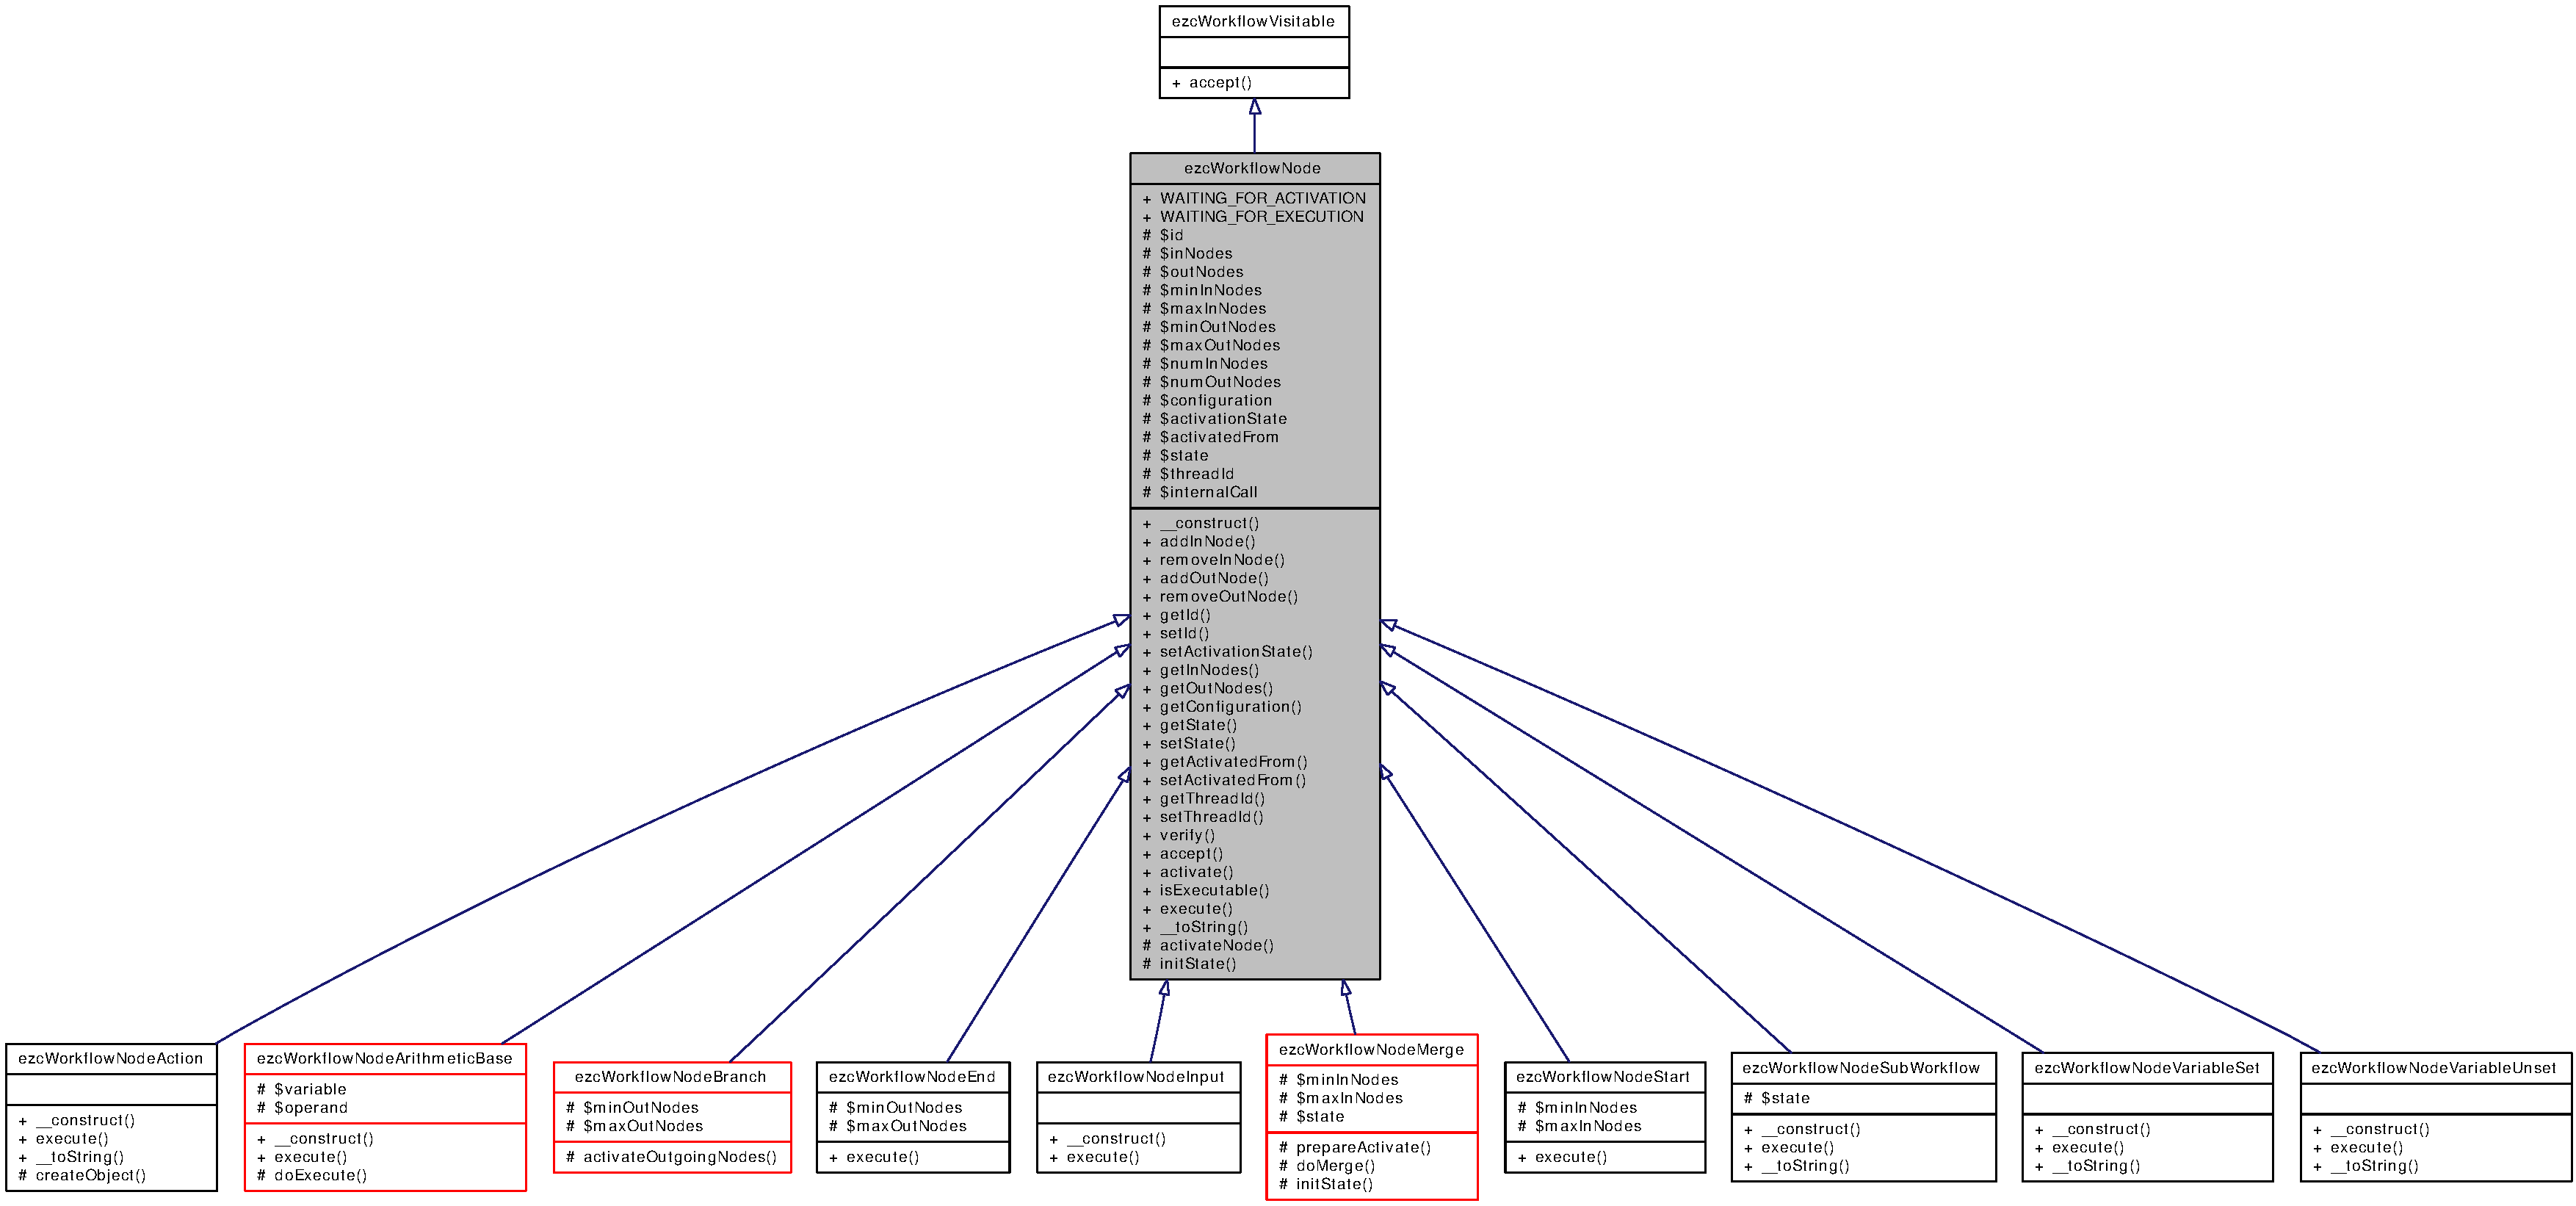
\includegraphics[angle=90,width=10cm]{figures/WorkflowNode}\\[5mm]
\end{center}
\caption{The \texttt{ezcWorkflowNode} class and its subclasses}
\label{classezcWorkflowNode}
\end{figure}

\subsection{Start and End Nodes}

\subsubsection{ezcWorkflowNodeStart}

\emph{Incoming Nodes: 0}\\
\emph{Outgoing Nodes: 1}\\

An object of the \texttt{ezcWorkflowNodeStart} class (see
Figure~\ref{classezcWorkflowNode}) represents the one and only start node of a
workflow. The execution of the workflow starts here.

Creating an object of the \texttt{ezcWorkflow} automatically creates the
start node for this new workflow.

\begin{lstlisting}[language=PHP]
$workflow = new ezcWorkflow( 'Name' );
$workflow->startNode; // This property holds the ezcWorkflowNodeStart object.
\end{lstlisting}

\subsubsection{ezcWorkflowNodeEnd}

\emph{Incoming Nodes: 1}\\
\emph{Outgoing Nodes: 0}\\

An object of the \texttt{ezcWorkflowNodeEnd} class (see
Figure~\ref{classezcWorkflowNode}) represents an end node of a workflow. A
workflow must have at least one end node. The execution of the workflow ends
when an end node is reached.

Creating an object of the \texttt{ezcWorkflow} automatically creates a default
end node for this new workflow.

\begin{lstlisting}[language=PHP]
$workflow = new ezcWorkflow( 'Name' );
$workflow->endNode; // This property holds an ezcWorkflowNodeEnd object.
\end{lstlisting}

\subsubsection{ezcWorkflowNodeCancel}

\emph{Incoming Nodes: 1}\\
\emph{Outgoing Nodes: 0..1}\\

The \texttt{ezcWorkflowNodeCancel} class implements the
\emph{Cancel Case} workflow pattern.

\begin{lstlisting}[language=PHP]
$workflow = new ezcWorkflow( 'Name' );
$workflow->endNode = new ezcWorkflowNodeCancel;
\end{lstlisting}

As soon as a node of the \texttt{ezcWorkflowNodeCancel} type is activated, the
complete workflow instance is removed. This includes currently executing nodes,
those which may execute at some future time and all parent and sub-workflows.
The workflow instance is recorded as having completed unsuccessfully.

\subsubsection{ezcWorkflowNodeFinally}

\emph{Incoming Nodes: 0}\\
\emph{Outgoing Nodes: 1}\\

An object of the \texttt{ezcWorkflowNodeFinally} class (see
Figure~\ref{classezcWorkflowNode}) represents the start node of a sequence of
final activities that is executed when a workflow execution is cancelled.

Creating an object of the \texttt{ezcWorkflow} class automatically creates the
finally node for this new workflow.

\begin{lstlisting}[language=PHP]
$workflow = new ezcWorkflow( 'Name' );
$workflow->endNode = new ezcWorkflowNodeCancel;
$workflow->finallyNode->addOutNode( /* ... */ );
\end{lstlisting}

\subsection{ezcWorkflowNodeAction}

\emph{Incoming Nodes: 1}\\
\emph{Outgoing Nodes: 1}\\

An object of the \texttt{ezcWorkflowNodeAction} class (see
Figure~\ref{classezcWorkflowNode}) represents an activity node. When the node
is reached, the business logic that is implemented by the associated
\emph{service object} is executed.

\begin{lstlisting}[language=PHP]
class MyAction implements ezcWorkflowServiceObject
{
    public function execute( ezcWorkflowExecution $execution )
    {
        // ...
    }

    public function __toString()
    {
        // ...
    }
}

$action = new ezcWorkflowNodeAction( 'MyAction' );
\end{lstlisting}

\subsection{ezcWorkflowNodeSubWorkflow}

\emph{Incoming Nodes: 1}\\
\emph{Outgoing Nodes: 1}\\

An object of the \texttt{ezcWorkflowNodeSubWorkflow} class (see
Figure~\ref{classezcWorkflowNode}) represents a sub-workflow. When the node
is reached, the specified sub-workflow is started. The workflow is suspended
until the sub-workflow has finished executing.

\begin{lstlisting}[language=PHP]
$subWorkflow = new ezcWorkflow( 'Sub-Workflow Name' );
// ...

$subWorkflow = new ezcWorkflowNodeSubWorkflow( 'Sub-Workflow Name' );
\end{lstlisting}

Workflow variables can be passed from the parent workflow to the
child worflow and vice versa. The example below creates a sub-workflow
node that passes the parent execution's variable \texttt{x} to the variable
\texttt{y} in the child execution when the sub-workflow is started. When it
ends, the child execution's \texttt{y} variable is passed to the parent
execution as \texttt{z}.

\begin{lstlisting}[language=PHP]
$subWorkflow = new ezcWorkflow( 'Sub-Workflow Name' );
// ...

$subWorkflow = new ezcWorkflowNodeSubWorkflow(
  array(
    'workflow'  => 'IncrementVariable',
    'variables' => array(
      'in' => array(
        'x' => 'y'
      ),
      'out' => array(
        'y' => 'z'
      )
    )
  )
);
\end{lstlisting}

\subsection{Workflow Variables}

\subsubsection{ezcWorkflowNodeInput}

\emph{Incoming Nodes: 1}\\
\emph{Outgoing Nodes: 1}\\

An object of the \texttt{ezcWorkflowNodeInput} class (see
Figure~\ref{classezcWorkflowNode}) represents an input node. When the node is
reached, the workflow engine will suspend the workflow execution if the
specified input data is not available (first activation). While the workflow
is suspended, the application that embeds the workflow engine may supply the
input data and resume the workflow execution (second activation of the input
node). Input data is stored in a workflow variable.

\subsubsection{ezcWorkflowNodeVariableSet}

\emph{Incoming Nodes: 1}\\
\emph{Outgoing Nodes: 1}\\

An object of the \texttt{ezcWorkflowNodeVariableSet} class sets a specified
workflow variable to a given value.

\begin{lstlisting}[language=PHP]
$set = new ezcWorkflowNodeVariableSet(
  array( 'variable name' => $value )
);
\end{lstlisting}

\subsubsection{ezcWorkflowNodeVariableUnset}

\emph{Incoming Nodes: 1}\\
\emph{Outgoing Nodes: 1}\\

An object of the \texttt{ezcWorkflowNodeVariableUnset} class unsets a
specified workflow variable.

\begin{lstlisting}[language=PHP]
$unset = new ezcWorkflowNodeVariableUnset( 'variable name' );
\end{lstlisting}

\begin{figure}[hbt]
\begin{center}
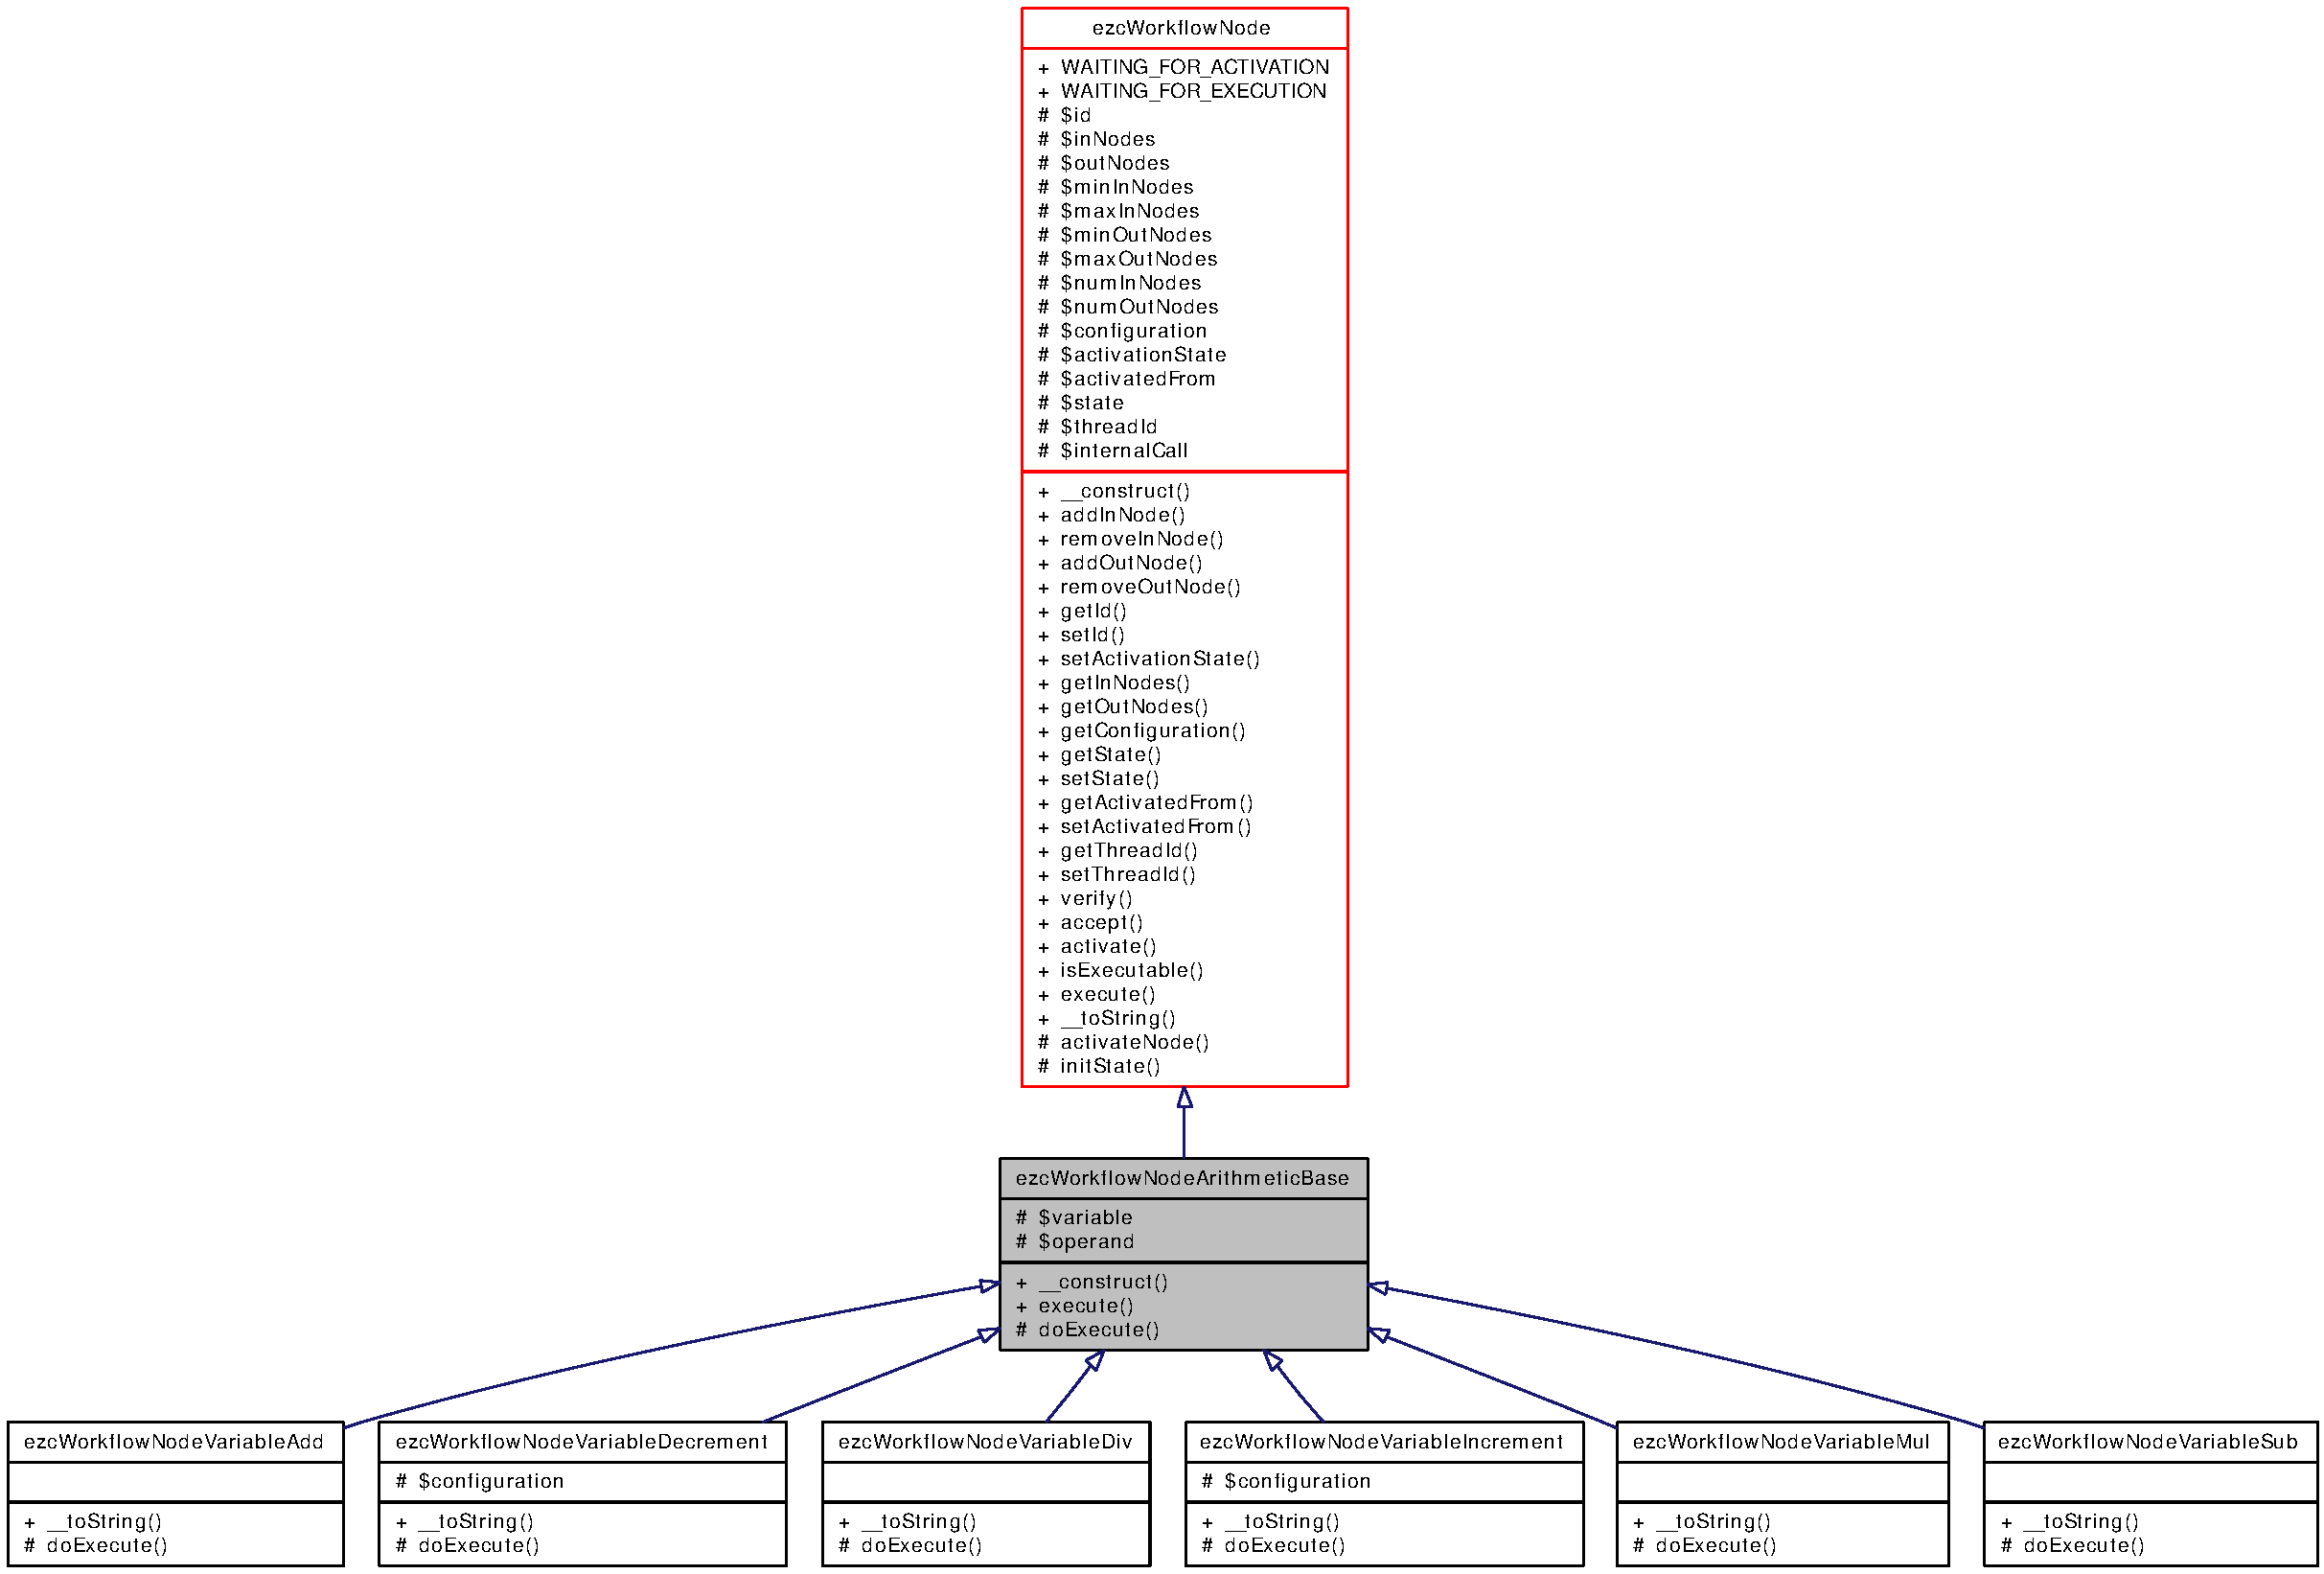
\includegraphics[width=16cm]{figures/WorkflowNodeArithmeticBase}\\[5mm]
\end{center}
\caption{The \texttt{ezcWorkflowNodeArithmeticBase} class and its subclasses}
\label{classezcWorkflowNodeArithmeticBase}
\end{figure}

\subsubsection{ezcWorkflowNodeVariableAdd}

\emph{Incoming Nodes: 1}\\
\emph{Outgoing Nodes: 1}\\

An object of the \texttt{ezcWorkflowNodeVariableAdd} class adds a given value,
either a constant or the value of another workflow variable, to a specified
workflow variable.

\begin{lstlisting}[language=PHP]
$add = new ezcWorkflowNodeVariableAdd(
  array( 'name' => 'variable name', 'value' => $value )
);
\end{lstlisting}

When \texttt{\$value} is a string, the value of the variable identified by
that string is used.

\subsubsection{ezcWorkflowNodeVariableSub}

\emph{Incoming Nodes: 1}\\
\emph{Outgoing Nodes: 1}\\

An object of the \texttt{ezcWorkflowNodeVariableSub} class subtracts a given
value, either a constant or the value of another workflow variable, from a
specified workflow variable.

\begin{lstlisting}[language=PHP]
$sub = new ezcWorkflowNodeVariableSub(
  array( 'name' => 'variable name', 'value' => $value )
);
\end{lstlisting}

When \texttt{\$value} is a string, the value of the variable identified by
that string is used.

\subsubsection{ezcWorkflowNodeVariableMul}

\emph{Incoming Nodes: 1}\\
\emph{Outgoing Nodes: 1}\\

An object of the \texttt{ezcWorkflowNodeVariableMul} class multiplies a specified
workflow variable with a given value, either a constant or the value of another
workflow variable.

\begin{lstlisting}[language=PHP]
$mul = new ezcWorkflowNodeVariableMul(
  array( 'name' => 'variable name', 'value' => $value )
);
\end{lstlisting}

When \texttt{\$value} is a string, the value of the variable identified by
that string is used.

\subsubsection{ezcWorkflowNodeVariableDiv}

\emph{Incoming Nodes: 1}\\
\emph{Outgoing Nodes: 1}\\

An object of the \texttt{ezcWorkflowNodeVariableDiv} class divides a specified
workflow variable by a given value, either a constant or the value of another
workflow variable.

\begin{lstlisting}[language=PHP]
$div = new ezcWorkflowNodeVariableDiv(
  array( 'name' => 'variable name', 'value' => $value )
);
\end{lstlisting}

When \texttt{\$value} is a string, the value of the variable identified by
that string is used.

\subsubsection{ezcWorkflowNodeVariableIncrement}

\emph{Incoming Nodes: 1}\\
\emph{Outgoing Nodes: 1}\\

An object of the \texttt{ezcWorkflowNodeVariableIncrement} class increments
the value of a specified workflow variable.

\begin{lstlisting}[language=PHP]
$inc = new ezcWorkflowNodeVariableIncrement( 'variable name' );
\end{lstlisting}

\subsubsection{ezcWorkflowNodeVariableDecrement}

\emph{Incoming Nodes: 1}\\
\emph{Outgoing Nodes: 1}\\

An object of the \texttt{ezcWorkflowNodeVariableDecrement} class decrements
the value of a specified workflow variable.

\begin{lstlisting}[language=PHP]
$dec = new ezcWorkflowNodeVariableDecrement( 'variable name' );
\end{lstlisting}

\subsection{Workflow Patterns}

\subsubsection{ezcWorkflowNodeParallelSplit}

\emph{Incoming Nodes: 1}\\
\emph{Outgoing Nodes: 2 \dots *}\\

The \texttt{ezcWorkflowNodeParallelSplit} class implements the
\emph{Parallel Split} workflow pattern.

\begin{figure}[hbt]
\begin{center}
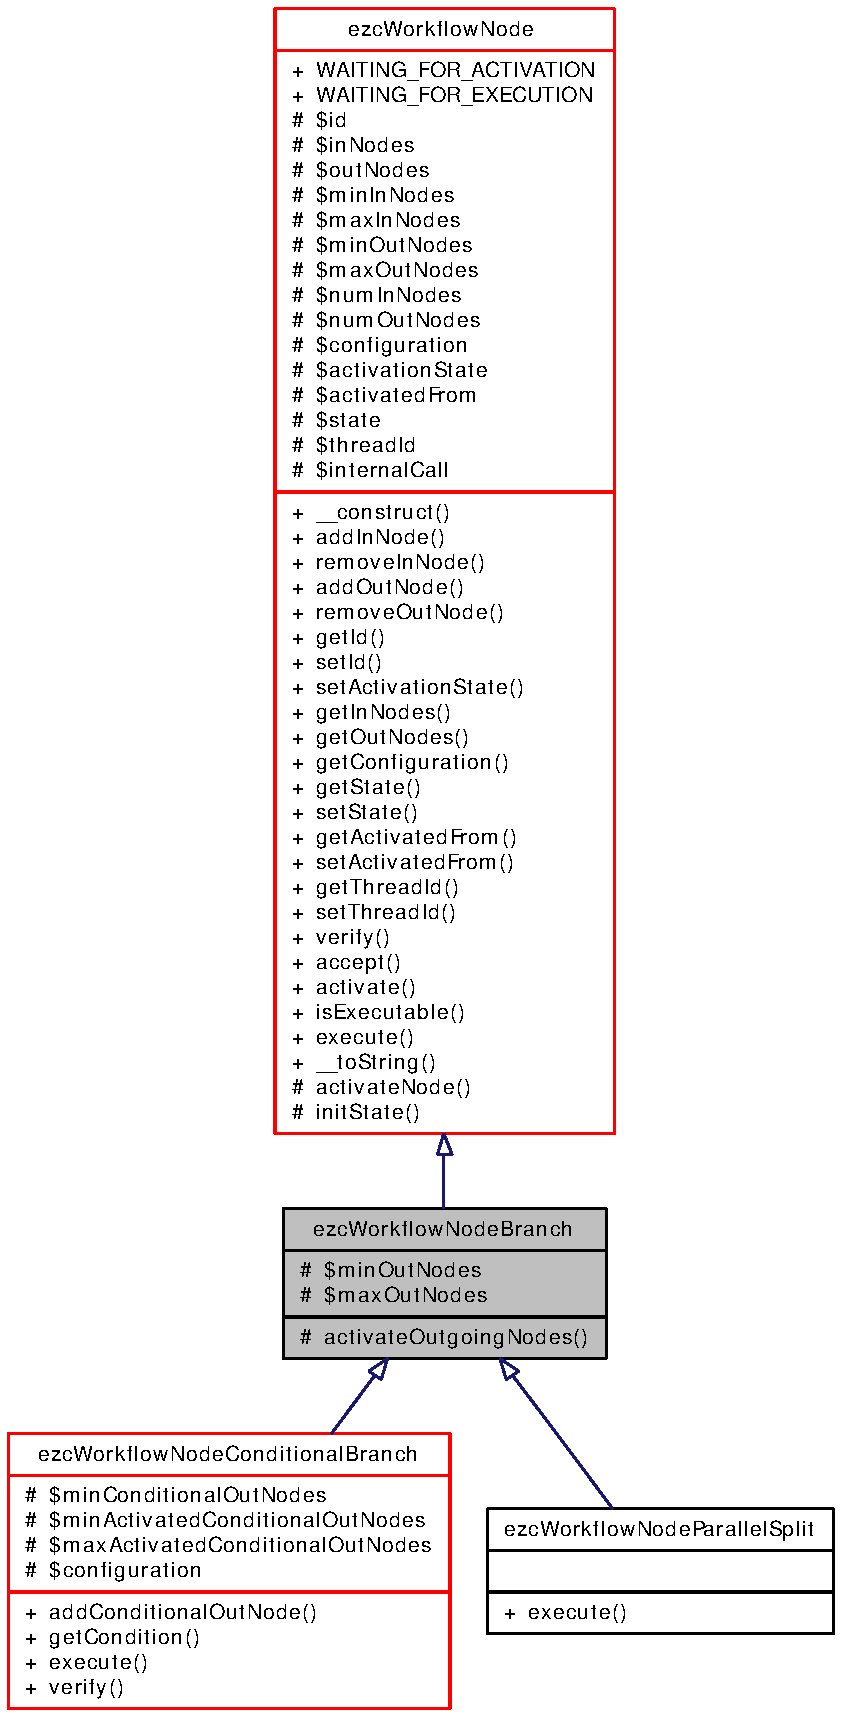
\includegraphics[width=10cm]{figures/WorkflowNodeBranch}\\[5mm]
\end{center}
\caption{The \texttt{ezcWorkflowNodeBranch} class and its subclasses}
\label{classezcWorkflowNodeBranch}
\end{figure}

\subsubsection{ezcWorkflowNodeSynchronization}

\emph{Incoming Nodes: 2 \dots *}\\
\emph{Outgoing Nodes: 1}\\

The \texttt{ezcWorkflowNodeSynchronization} class implements the
\emph{Synchronization} workflow pattern.

\begin{figure}[hbt]
\begin{center}
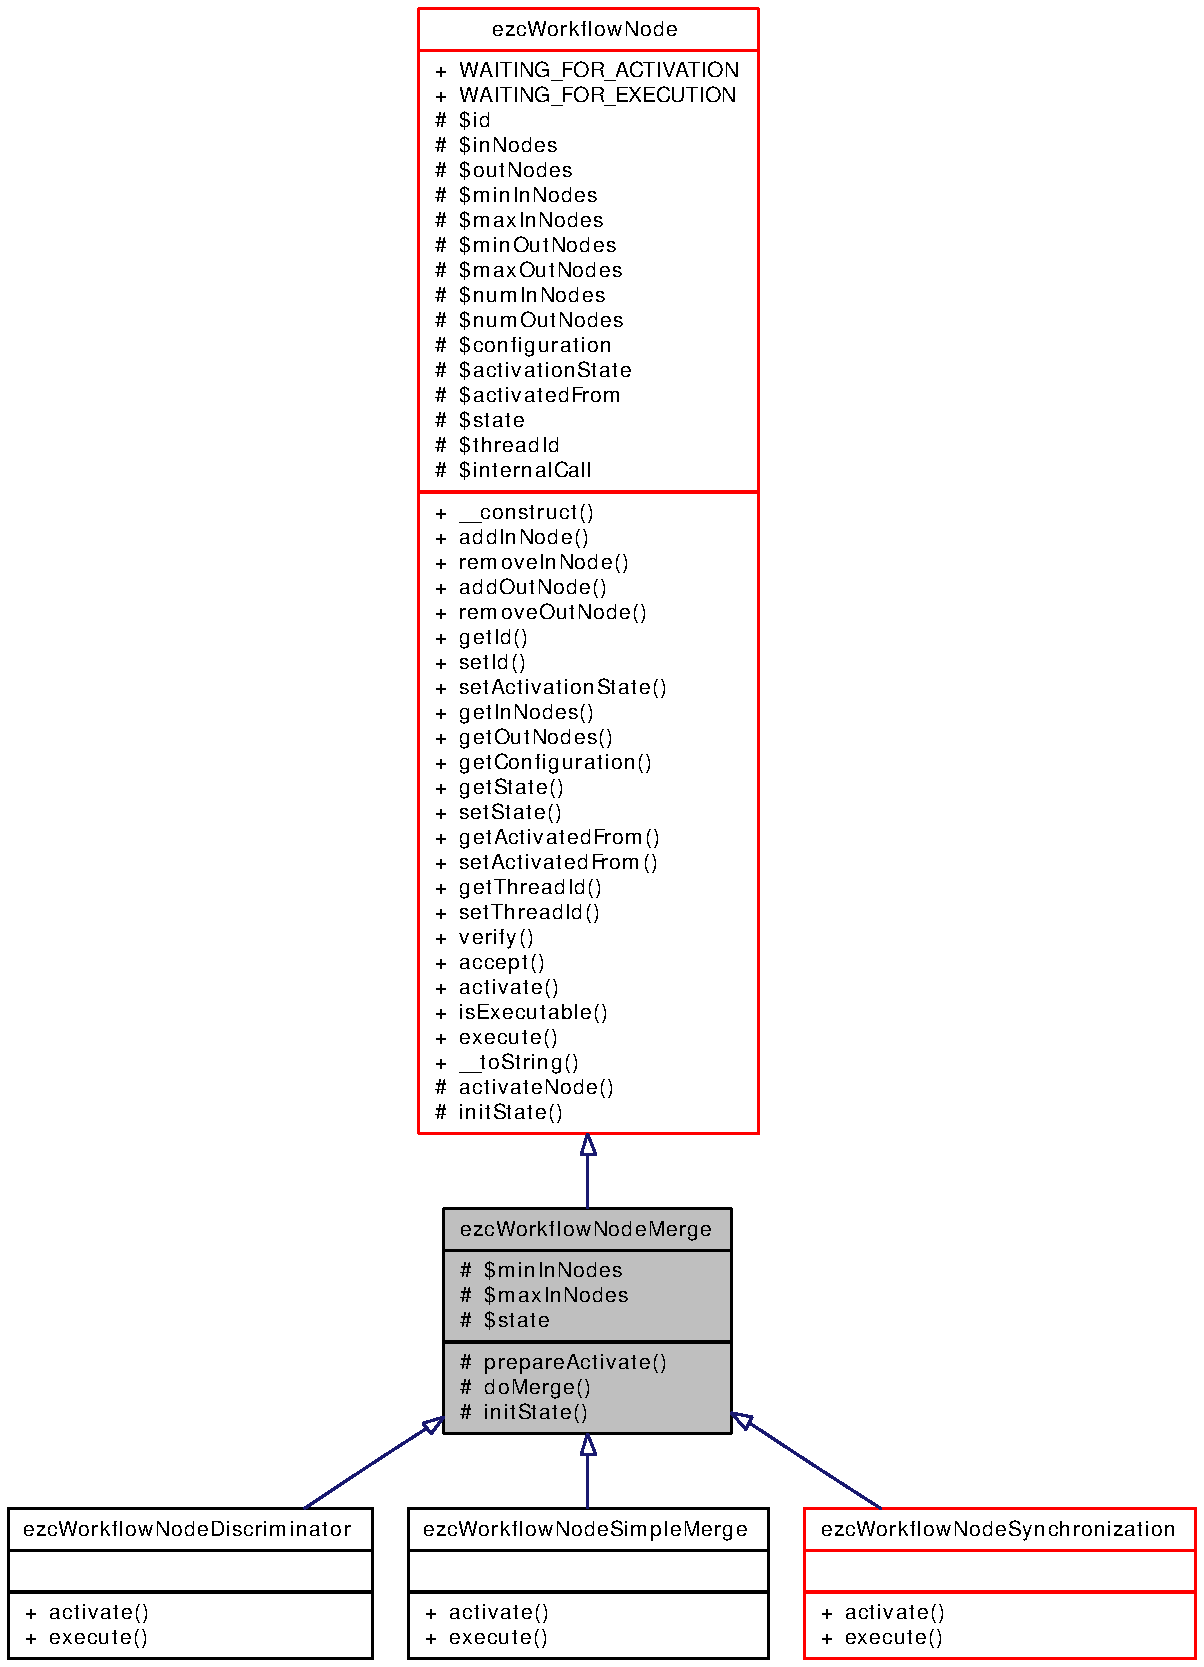
\includegraphics[width=10cm]{figures/WorkflowNodeMerge}\\[5mm]
\end{center}
\caption{The \texttt{ezcWorkflowNodeMerge} class and its subclasses}
\label{classezcWorkflowNodeMerge}
\end{figure}

\begin{figure}[hbt]
\begin{center}
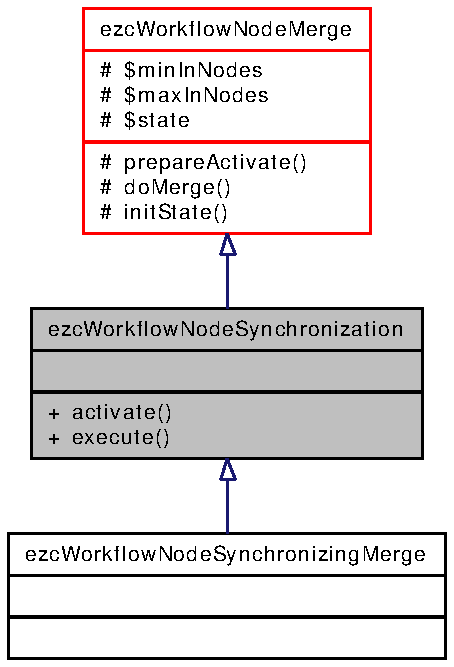
\includegraphics[width=6cm]{figures/WorkflowNodeSynchronization}\\[5mm]
\end{center}
\caption{The \texttt{ezcWorkflowNodeSynchronization} class and its subclasses}
\label{classezcWorkflowNodeSynchronization}
\end{figure}

\subsubsection{ezcWorkflowNodeExclusiveChoice}

\emph{Incoming Nodes: 1}\\
\emph{Outgoing Nodes: 2 \dots *}\\

The \texttt{ezcWorkflowNodeExclusiveChoice} class implements the
\emph{Exclusive Choice} workflow pattern.

\begin{figure}[hbt]
\begin{center}
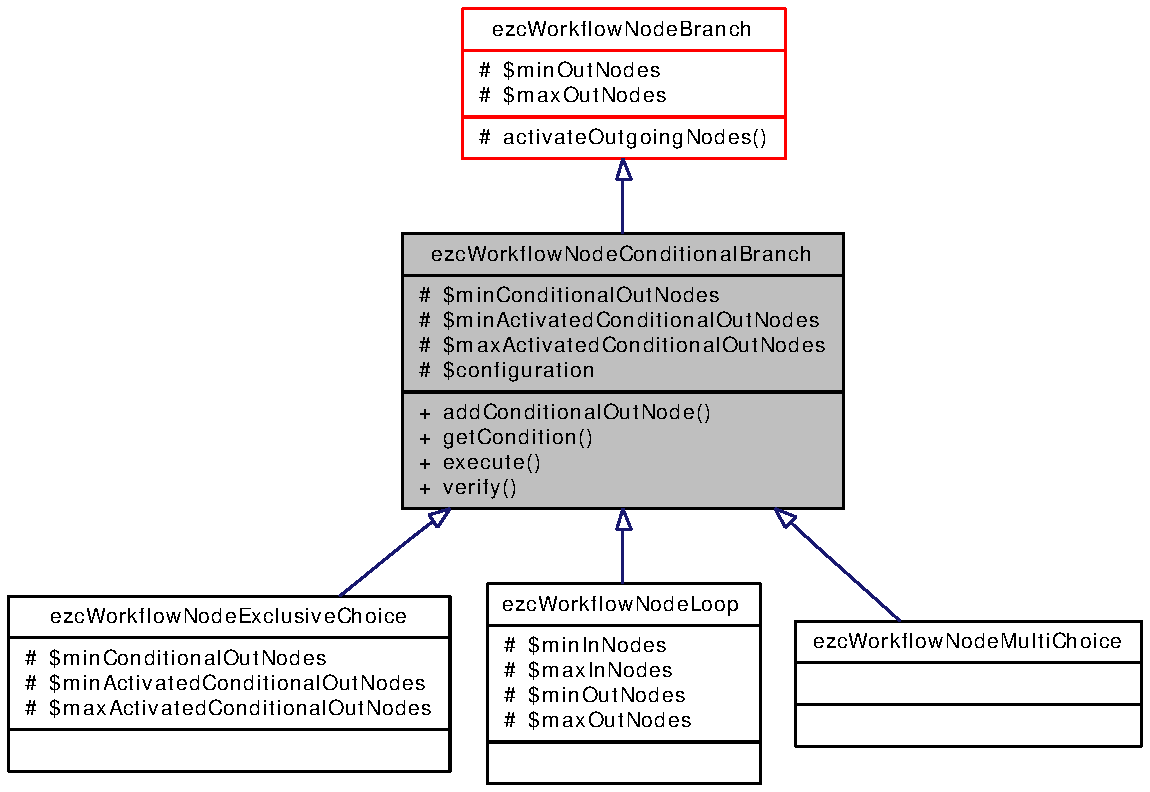
\includegraphics[width=8cm]{figures/WorkflowNodeConditionalBranch}\\[5mm]
\end{center}
\caption{The \texttt{ezcWorkflowNodeConditionalBranch} class and its subclasses}
\label{classezcWorkflowNodeConditionalBranch}
\end{figure}

\subsubsection{ezcWorkflowNodeSimpleMerge}

\emph{Incoming Nodes: 2 \dots *}\\
\emph{Outgoing Nodes: 1}\\

The \texttt{ezcWorkflowNodeSimpleMerge} class implements the \emph{Simple Merge}
workflow pattern.

\subsubsection{ezcWorkflowNodeLoop}

\emph{Incoming Nodes: 2}\\
\emph{Outgoing Nodes: 2}\\

The \texttt{ezcWorkflowNodeLoop} class is a specialization of the
\texttt{ezcWorkflowNodeExclusiveChoice} class and may be used to conveniently
express loops.

\begin{lstlisting}[language=PHP]
$workflow = new ezcWorkflow( 'IncrementingLoop' );

$set  = new ezcWorkflowNodeVariableSet( array( 'i' => 1 ) );
$step = new ezcWorkflowNodeVariableIncrement( 'i' );

$break = new ezcWorkflowConditionVariable(
  'i', new ezcWorkflowConditionIsEqual( 10 )
);

$continue = new ezcWorkflowConditionVariable(
  'i', new ezcWorkflowConditionIsLessThan( 10 )
);

$workflow->startNode->addOutNode( $set );

$loop = new ezcWorkflowNodeLoop;
$loop->addInNode( $set )
       addInNode( $step )
       addConditionalOutNode( $continue, $step )
       addConditionalOutNode( $break, $workflow->endNode );
\end{lstlisting}

The code above is equivalent to a \texttt{for}-loop that iterates the variable
\texttt{i} from \texttt{1} to \texttt{10}.

\subsubsection{ezcWorkflowNodeMultiChoice}

\emph{Incoming Nodes: 1}\\
\emph{Outgoing Nodes: 2 \dots *}\\

The \texttt{ezcWorkflowNodeMultiChoice} class implements the \emph{Multi-Choice}
workflow pattern.

\subsubsection{ezcWorkflowNodeSynchronizingMerge}

\emph{Incoming Nodes: 2 \dots *}\\
\emph{Outgoing Nodes: 1}\\

The \texttt{ezcWorkflowNodeSynchronizingMerge} class implements the
\emph{Synchronizing Merge} workflow pattern.

\subsubsection{ezcWorkflowNodeDiscriminator}

\emph{Incoming Nodes: 2 \dots *}\\
\emph{Outgoing Nodes: 1}\\

The \texttt{ezcWorkflowNodeDiscriminator} class implements the
\emph{Discriminator} workflow pattern.


\section{Condition Classes}
\label{section-ConditionClasses}

The \texttt{ezcWorkflowCondition} classes can be used to express branch
conditions and input validation.

\subsection{Variable Access}

\subsubsection{ezcWorkflowConditionVariable}

An object of the \texttt{ezcWorkflowConditionVariable} class decorates another\\
\texttt{ezcWorkflowCondition} object and applies it condition to a workflow
variable.

\begin{lstlisting}[language=PHP]
$condition = new ezcWorkflowConditionVariable(
  'foo', new ezcWorkflowConditionIsTrue
);
\end{lstlisting}

\subsubsection{ezcWorkflowConditionVariables}

An object of the \texttt{ezcWorkflowConditionVariables} class decorates an\\
\texttt{ezcWorkflowConditionComparison} object and applies it to two workflow
variables.

\begin{lstlisting}[language=PHP]
$condition = new ezcWorkflowConditionVariables(
  'foo', 'bar', new ezcWorkflowConditionIsEqual
);
\end{lstlisting}

\subsection{Boolean Expressions}

\subsubsection{ezcWorkflowConditionNot}

An object of the \texttt{ezcWorkflowConditionNot} class decorates an
\texttt{ezcWorkflowCondition} object and negates its expression.

\begin{lstlisting}[language=PHP]
$notNondition = new ezcWorkflowConditionNot( $condition );
\end{lstlisting}

\subsubsection{ezcWorkflowConditionAnd}

An object of the \texttt{ezcWorkflowConditionAnd} class represents a
boolean \emph{AND} expression. It can hold an arbitrary number of
\texttt{ezcWorkflowCondition} objects.

\begin{lstlisting}[language=PHP]
$and = new ezcWorkflowConditionAnd( array( $condition, ... ) );
\end{lstlisting}

\subsubsection{ezcWorkflowConditionOr}

An object of the \texttt{ezcWorkflowConditionOr} class represents a
boolean \emph{OR} expression. It can hold an arbitrary number of
\texttt{ezcWorkflowCondition} objects.

\begin{lstlisting}[language=PHP]
$or = new ezcWorkflowConditionOr( array( $condition, ... ) );
\end{lstlisting}

\subsubsection{ezcWorkflowConditionXor}

An object of the \texttt{ezcWorkflowConditionXor} class represents a
boolean \emph{XOR} expression. It can hold an arbitrary number of
\texttt{ezcWorkflowCondition} objects.

\begin{lstlisting}[language=PHP]
$xor = new ezcWorkflowConditionXor( array( $condition, ... ) );
\end{lstlisting}

\subsection{Comparisons}

\subsubsection{ezcWorkflowConditionIsTrue}

The condition represented by an \texttt{ezcWorkflowConditionIsTrue} object
evaluates to \texttt{true} when the associated workflow variable has the
value \texttt{true}.

\begin{lstlisting}[language=PHP]
$condition = new ezcWorkflowConditionVariable(
  'variable name',
  new ezcWorkflowConditionIsTrue
);
\end{lstlisting}

\subsubsection{ezcWorkflowConditionIsFalse}

The condition represented by an \texttt{ezcWorkflowConditionIsFalse} object
evaluates to \texttt{true} when the associated workflow variable has the
value \texttt{false}.

\begin{lstlisting}[language=PHP]
$condition = new ezcWorkflowConditionVariable(
  'variable name',
  new ezcWorkflowConditionIsFalse
);
\end{lstlisting}

\subsubsection{ezcWorkflowConditionIsEqual}

The condition represented by an \texttt{ezcWorkflowConditionIsEqual} object
evaluates to \texttt{true} when the associated workflow variable is equal to
the comparison value.

\begin{lstlisting}[language=PHP]
$condition = new ezcWorkflowConditionVariable(
  'variable name',
  new ezcWorkflowConditionIsEqual( $comparisonValue )
);
\end{lstlisting}

\subsubsection{ezcWorkflowConditionIsNotEqual}

The condition represented by an \texttt{ezcWorkflowConditionIsNotEqual} object
evaluates to \texttt{true} when the associated workflow variable is not equal
to the comparison value.

\begin{lstlisting}[language=PHP]
$condition = new ezcWorkflowConditionVariable(
  'variable name',
  new ezcWorkflowConditionIsNotEqual( $comparisonValue )
);
\end{lstlisting}

\subsubsection{ezcWorkflowConditionIsGreaterThan}

The condition represented by an \texttt{ezcWorkflowConditionIsGreaterThan}
object evaluates to \texttt{true} when the associated workflow variable is
greater than the comparison value.

\begin{lstlisting}[language=PHP]
$condition = new ezcWorkflowConditionVariable(
  'variable name',
  new ezcWorkflowConditionIsGreaterThan( $comparisonValue )
);
\end{lstlisting}

\subsubsection{ezcWorkflowConditionIsEqualOrGreaterThan}

The condition represented by an \texttt{ezcWorkflowConditionIsEqualOrGreaterThan}
object evaluates to \texttt{true} when the associated workflow variable is
equal or greater than the comparison value.

\begin{lstlisting}[language=PHP]
$condition = new ezcWorkflowConditionVariable(
  'variable name',
  new ezcWorkflowConditionIsEqualOrGreaterThan( $comparisonValue )
);
\end{lstlisting}

\subsubsection{ezcWorkflowConditionIsLessThan}

The condition represented by an \texttt{ezcWorkflowConditionIsLessThan}
object evaluates to \texttt{true} when the associated workflow variable is
less than the comparison value.

\begin{lstlisting}[language=PHP]
$condition = new ezcWorkflowConditionVariable(
  'variable name',
  new ezcWorkflowConditionIsLessThan( $comparisonValue )
);
\end{lstlisting}

\subsubsection{ezcWorkflowConditionIsEqualOrLessThan}

The condition represented by an \texttt{ezcWorkflowConditionIsEqualOrLessThan}
object evaluates to \texttt{true} when the associated workflow variable is
equal or less than the comparison value.

\begin{lstlisting}[language=PHP]
$condition = new ezcWorkflowConditionVariable(
  'variable name',
  new ezcWorkflowConditionIsEqualOrLessThan( $comparisonValue )
);
\end{lstlisting}

\subsection{Types}

\subsubsection{ezcWorkflowConditionIsAnything}

The condition represented by an \texttt{ezcWorkflowConditionIsAnything} object
always evaluates to \texttt{true}.

\begin{lstlisting}[language=PHP]
$condition = new ezcWorkflowConditionVariable(
  'variable name',
  new ezcWorkflowConditionIsAnything
);
\end{lstlisting}

\subsubsection{ezcWorkflowConditionIsArray}

The condition represented by an \texttt{ezcWorkflowConditionIsArray}
object evaluates to \texttt{true} when the associated workflow variable is
an array.

\begin{lstlisting}[language=PHP]
$condition = new ezcWorkflowConditionVariable(
  'variable name',
  new ezcWorkflowConditionIsArray
);
\end{lstlisting}

\subsubsection{ezcWorkflowConditionIsBool}

The condition represented by an \texttt{ezcWorkflowConditionIsBool}
object evaluates to \texttt{true} when the associated workflow variable is
a boolean.

\begin{lstlisting}[language=PHP]
$condition = new ezcWorkflowConditionVariable(
  'variable name',
  new ezcWorkflowConditionIsBool
);
\end{lstlisting}

\subsubsection{ezcWorkflowConditionIsFloat}

The condition represented by an \texttt{ezcWorkflowConditionIsFloat}
object evaluates to \texttt{true} when the associated workflow variable is
a float.

\begin{lstlisting}[language=PHP]
$condition = new ezcWorkflowConditionVariable(
  'variable name',
  new ezcWorkflowConditionIsFloat
);
\end{lstlisting}

\subsubsection{ezcWorkflowConditionIsInteger}

The condition represented by an \texttt{ezcWorkflowConditionIsInteger}
object evaluates to \texttt{true} when the associated workflow variable is
an integer.

\begin{lstlisting}[language=PHP]
$condition = new ezcWorkflowConditionVariable(
  'variable name',
  new ezcWorkflowConditionIsInteger
);
\end{lstlisting}

\subsubsection{ezcWorkflowConditionIsObject}

The condition represented by an \texttt{ezcWorkflowConditionIsObject}
object evaluates to \texttt{true} when the associated workflow variable is
an object.

\begin{lstlisting}[language=PHP]
$condition = new ezcWorkflowConditionVariable(
  'variable name',
  new ezcWorkflowConditionIsObject
);
\end{lstlisting}

\subsubsection{ezcWorkflowConditionIsString}

The condition represented by an \texttt{ezcWorkflowConditionIsString}
object evaluates to \texttt{true} when the associated workflow variable is
a string

\begin{lstlisting}[language=PHP]
$condition = new ezcWorkflowConditionVariable(
  'variable name',
  new ezcWorkflowConditionIsString
);
\end{lstlisting}

\begin{thebibliography}{99999}

\bibitem[AIIM]{AIIM} Association for Information and Image Management (AIIM).
\emph{What is ECM?}\\
\url{http://www.aiim.org/about-ecm.asp}

\bibitem[ARK03]{ARK03} Atul Ravi Khemuka.
\emph{Workflow Modeling Using Finite Automata}.
PhD Thesis, Department of Industrial and Management Engineering, College of Engineering, University of South Florida, USA, 2003.

\bibitem[BK03]{BK03} Bartosz Kiepuszewski.
\emph{Expressiveness and Suitability of Languages for Control Flow Modelling in Workflows}.
PhD Thesis, Faculty of Information Technology, Queensland University of Technology, Australia, 2003.

\bibitem[DAM01]{DAM01} Dragos-Anton Manolescu.
\emph{Micro-Workflow: A Workflow Architecture Supporting Compositional Object-Oriented Software Development}.
PhD Thesis, Department of Computer Science, University of Illinois at Urbana-Champaign, USA, 2001.

\bibitem[DG95]{DG95} Dimitrios Georgakopoulos and Mark F. Hornick and Amit P. Sheth.
\emph{An Overview of Workflow Management: From Process Modeling to Workflow Automation Infrastructure}.
In: Distributed and Parallel Databases, Volume 3, Number 2, Pages 119--153, 1995.

\bibitem[DQZ01]{DQZ01} Da-Qian Zhang and Kang Zhang and Jiannong Cao.
\emph{A Context-Sensitive Graph Grammar Formalism for the Specification of Visual Languages}.
In: The Computer Journal, Volume 33, Number 3, Pages 186--200, 2001.

\bibitem[DS06]{DS06} Douglas C. Schmidt.
\emph{Model-Driven Engineering}.
In: IEEE Computer, Volume 39, Number 2, Pages 25--31, 2006.

\bibitem[FB96]{FB96} Frank Buschmann and Regine Meunier and Hans Rohnert and Peter Sommerlad and Michael Stahl.
\emph{Pattern-Oriented Software Architecture -- A System of Patterns}.
John Wiley \& Sons, 1996.

\bibitem[FG02]{FG02} Florent Guillaume.
\emph{Trying to unify Entity-based and Activity-based workflows}.\\
\url{http://wiki.zope.org/zope3/TryingToUnifiyWorkflowConcepts}

\bibitem[GF03]{GF03} Garland Foster and Richard Moore and Eduardo Polidor.
\emph{Galaxia: An Open Source Workflow Engine for Tiki}\\
\url{http://workflow.tikiwiki.org/tiki-index.php?page=GalaxiaConcepts}

\bibitem[GoF94]{GoF94} Erich Gamma and Richard Helm and Ralph Johnson and John Vlissides.
\emph{Design Patterns: Elements of Reusable Object-Oriented Software}.
Addison-Wesley, 1994.

\bibitem[JBOSS]{JBOSS} The JBoss Project.
\emph{JBoss jBPM: Workflow and BPM Made Practical}.\\
\url{http://docs.jboss.com/jbpm/v3/userguide/graphorientedprogramming.html}

\bibitem[JD01]{JD01} J�rg Desel and Gabriel Juh�s.
\emph{What Is a Petri Net?}.
In: Unifying Petri Nets: Advances in Petri Nets, Lecture Notes in Computer Science,
Volume 2128/2001, Springer, 2001.

\bibitem[JM01]{JM01} Jishnu Mukerji and Joaquin Miller.
\emph{MDA Guide}.\\
\url{http://www.omg.org/cgi-bin/apps/doc?omg/03-06-01.pdf}

\bibitem[KL97]{KL97} Karl J. Lieberherr.
\emph{Connections between Demeter/Adaptive Programming and Aspect-Oriented Programming (AOP)}.
College of Computer Science, Northeastern University, Boston, MA, USA, 1997.\\
\url{http://www.ccs.neu.edu/home/lieber/connection-to-aop.html}

\bibitem[MF05]{MF05} Martin Fowler.
\emph{Language Workbenches: The Killer-App for Domain Specific Languages?}
June, 2005.\\
\url{http://martinfowler.com/articles/languageWorkbench.html}

\bibitem[ML05]{ML05} Markus L�schnigg.
\emph{XML in Workflow Management Systems}.
Master's Thesis, Graz University of Technology, Austria, 2005.

\bibitem[OPENFLOW]{OPENFLOW} The OpenFlow Project.
\emph{OpenFlow: An Introduction}.\\
\url{http://www.openflow.it/wwwopenflow/Documentation/documentation/OpenFlowIntroduction/}

\bibitem[PM99]{PM99} Peter Muth and Jeanine Weisenfels and Michael Gillmann and Gerhard Weikum.
\emph{Integrating Light-Weight Workflow Management Systems within Existing Business Environments}.
In: Proceedings of the 15th International Conference on Data Engineering, March 1999, Sydney, Australia.

\bibitem[RA01]{RA01} Rob Allen.
\emph{Workflow: An Introduction}.
In: Workflow Handbook, Workflow Management Coalition, 2001.

\bibitem[RF00]{RF00} Robert E. Filman and Daniel P. Friedman.
\emph{Aspect-Oriented Programming is Quantification and Obliviousness}.
In: Proceedings of the Workshop on Advanced Separation of Concerns, OOPSLA 2000, October 2000, Minneapolis, USA.

\bibitem[SB05]{SB05} Sebastian Bergmann.
\emph{Professionelle Softwareentwicklung mit PHP 5}.
dpunkt.verlag, 2005.

\bibitem[SB06]{SB06} Sebastian Bergmann and G�nter Kniesel.
\emph{GAP: Generic Aspects for PHP}.
Third European Workshop on Aspects in Software, August 2006, University of Twente, Enschede, The Netherlands.

\bibitem[SF04]{SF04} S�rgio Fernandes and Jo�o Cachopo and Ant�nio Rito-Silva.
\emph{Supporting Evolution in Workflow Definition Languages}.
In: Proceedings of the 20th Conference on Current Trends in Theory and Practice of Computer Science (SOFSEM 2004), Springer-Verlag, 2004.

\bibitem[SH05]{SH05} Saphira Heijens.
\emph{Support for Workflow Administration and Monitoring in the YAWL Environment}.
Master Thesis, Vrije Universiteit, Amsterdam, The Netherlands, 2005.

\bibitem[TM04]{TM04} Tony Marston.
\emph{An Activity-Based Workflow Engine for PHP}.
September 2004.\\
\url{http://www.tonymarston.net/php-mysql/workflow.html}

\bibitem[TS04]{TS04} Thomas Schmidt.
\emph{Erweiterung und Integration des Open Source Workflow-Systems SWAMP am Beispiel eines Software-Wartungs-Prozesses}.
Diploma Thesis, Georg-Simon-Ohm-Fachhochschule, N�rnberg, Germany, 2004.

\bibitem[W3C07]{W3C07} World Wide Web Consortium.
\emph{XSL Transformations (XSLT) Version 2.0}.
W3C Recommendation, January 2007.\\
\url{http://www.w3.org/TR/2007/REC-xslt20-20070123/}

\bibitem[WA96]{WA96} W. M. P. van der Aalst.
\emph{Petri-net-based Workflow Management Software}.
In: Proceedings of the NFS Workshop on Workflow and Process Automation in Information Systems, May 1996, Athens, Georgia, USA.

\bibitem[WA04]{WA04} W. M. P. van der Aalst and L. Aldred and M. Dumas and A. H. M. ter Hofstede.
\emph{Design and Implementation of the YAWL System}.
In: Proceedings of the 16th International Conference on Advanced Information Systems Engineering (CAiSE 2004), June 2004, Riga, Latvia.

\bibitem[WfMC95]{WfMC95} Workflow Management Coalition.
\emph{The Workflow Reference Model}.
Document Number WFMC-TC-1003, 1995.

\bibitem[WfMC99]{WfMC99} Workflow Management Coalition.
\emph{Terminology and Glossary}.
Document Number WFMC-TC-1011, 1999.

\bibitem[WfMC05]{WfMC05} Workflow Management Coalition.
\emph{Workflow Process Definition Interface -- XML Process Definition Language (XPDL)}.
Document Number WFMC-TC-1025, 2005.

\end{thebibliography}


\end{appendix}

\end{document}

